\chapter[PB-2b CHWP evaluation]{PB-2b CHWP evaluation}
\label{ch:pb2b_chwp_evaluation}

The POLARBEAR-2b (PB-2b) cryogenic half-wave plate (CHWP) development began in 2014 as a list of requirements and a concept resembling the EBEX modulator design. During its maturation from that point until its deployment to Chile in 2020, the CHWP system underwent many iterations of design, build, test, and revise. Therefore, a thorough recount of the CHWP evaluation would include several testing campaigns of several distinct modulator incarnations. While such a comprehensive discussion would offer insight into the CHWP's maturation, we narrow the scope of this chapter to the development trajectory's endpoints.

%%%%%%%%%%%%%%%%%%%%%%%%%%%%%%%%
%%%%%%%%%%%%%%%%%%%%%%%%%%%%%%%%
%%%%%%%%%%%%%%%%%%%%%%%%%%%%%%%%

\section{Prototype evaluation}
\label{sec:pb2b_chwp_prototype}

In an effort to learn about the superconducting magnetic bearing (SMB), synchronous magnetic motors, encoder systems, and effective gripping strategies, we initiated the CHWP development with $\approx$~1.5~years of small-scale, $\sim$~120~mm prototyping. Figure~\ref{fig:chwp_prototype} show an advanced version of the prototype that was tested shortly before the PB-2b CHWP fabrication was launched. This prototype was built at Lawrence Berkeley National Laboratory (LBNL), in parallel with the receiver backend construction at University of California, San Diego (UCSD) and the optics-tube construction at UC Berkeley. While it somewhat resembles the design described in Chapter~\ref{ch:chwp_design}, the prototype has several hardware elements that were overhauled in the final design. Since the prototype was an integral part of the CHWP program, we discuss its evaluation in this section.

The prototype was evaluated in the CAPMAP dewar at LBNL and was cooled in the dewar eight times using the second stage of a Gifford-McMahon (GM) cooler. Each cooldown provided rapid feedback to the prototype evaluation process which led to hardware modifications, and the culmination of these tests formed the CHWP design presented in Chapter~\ref{ch:chwp_design}. We focus on the parts of the system that changed substantially between the small-scale and large-scale assemblies, highlighting the results of the prototype evaluation that led to those changes.

\begin{figure}[!t]
    \centering
    \subfloat[\label{fig:chwp_prototype:a}]{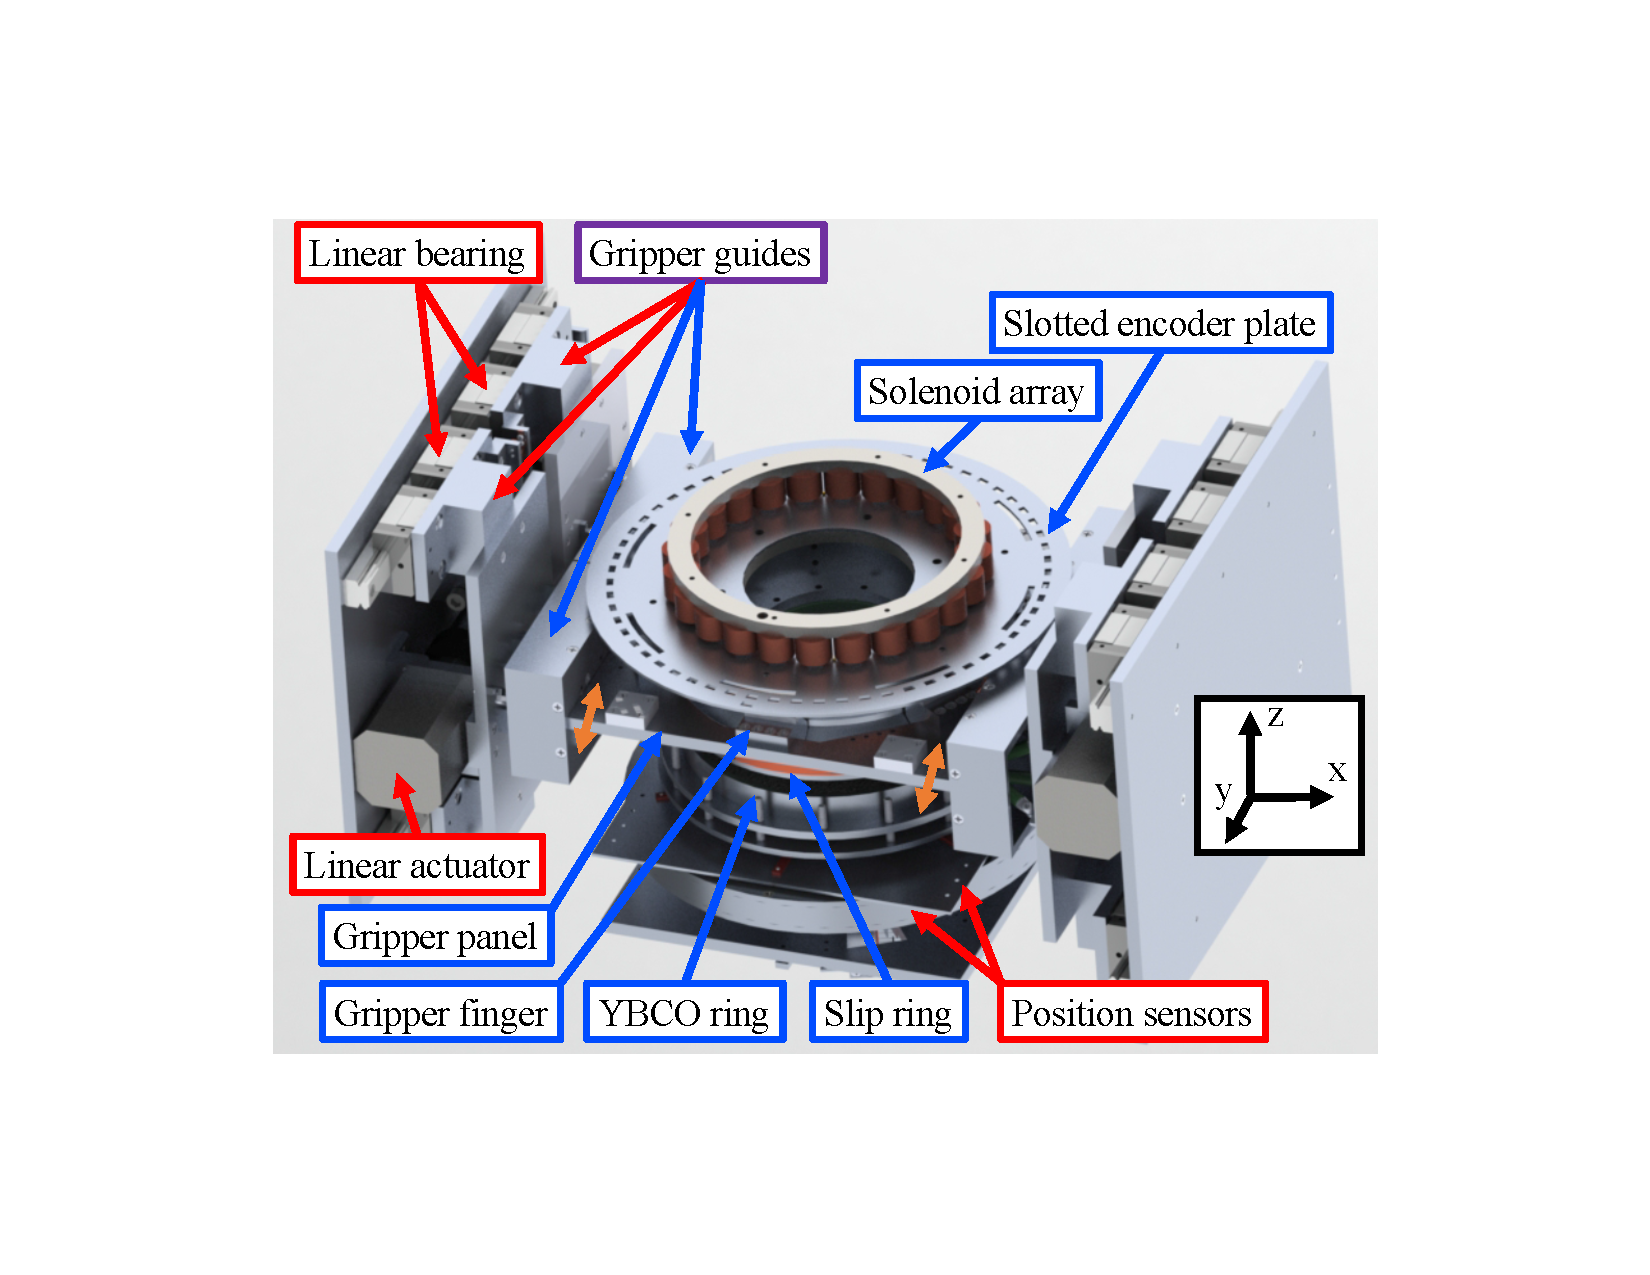
\includegraphics[width=0.48\linewidth, trim=4.5cm 3.5cm 4.5cm 3.5cm, clip]{CHWPEvaluation/Figures/chwp_prototype_cad.pdf}}
    \subfloat[\label{fig:chwp_prototype:b}]{\includegraphics[width=0.48\linewidth, trim=4.5cm 3.5cm 4.5cm 3.5cm, clip]{CHWPEvaluation/Figures/chwp_prototype_photo.pdf}}
    \caption[The CHWP prototype developed at LBNL.]{The CHWP prototype developed at LBNL prior to the construction of the PB-2b CHWP presented in Chapter~\ref{ch:chwp_design}. The CAD render (left) shows the prototype fully assembled, and the photo (right) shows a view from below of the prototype partially assembled in the CAPMAP dewar. The most prominent differences between the prototype and the PB-2b design is the gripper with vacuum-compatible bearings and motors, the existence of position sensors, which were removed from the final assembly.}
    \label{fig:chwp_prototype}
\end{figure}

The biggest modification between the prototype and full-scale CHWP is the gripping mechanism. The prototype's gripper is shown as part of Figure~\ref{fig:chwp_prototype} contains several differences to that of the PB-2b CHWP. The entire gripper mechanism, including the motors and linear bearings, are within the vacuum space. This choice was made to improve alignment between the 300~K and 50~K components but gave rise to more prohibitive problems, which we discuss below. The gripper assembly is composed of two subassemblies on either side of the CHWP along the $x$-direction that move two panels back and forth along the $y$-direction. Each gripper assembly has two 300~K linear bearings, two 300~K linear actuators, and two guides that move along these linear bearings and provide thermal isolation between the warm linear bearings and the cryogenic gripper panels. One motor on each panel is responsible for actuating each gripper panel along the $\pm$~$y$-direction, and each panel contains three gripper fingers oriented at (-45, 0, 45)~degrees with respect to the $y$-axis that contact a groove on the rotor stage. In a similar manner to that of the PB-2b CHWP, a slip ring is attached to the rotor stage and is used to read out a rotor thermometer via a slip-ring contact.

There were several issues with this prototype design that led to an overhauled design in the PB-2b CHWP system. First, the rotor is contacted by six gripper fingers on two moving panels, making it over-constrained and therefore prone to both poor heat sinking and poor alignment. Second, each gripper panel is also overconstrained, as it takes synchronized motion between two motors to actuate each panel along one direction. Therefore, if the motors are not perfectly synchronized, the panel becomes crooked and jammed. This failure mode was particularly problematic during CAPMAP testing, as it was difficult to diagnose stepper motor slippage without independent encoders on the gripper panels. Third, the prototype gripper relies on vacuum bearings and motors that are embedded into the CHWP assembly. Therefore, if there is a problem with either of these mechanical pieces---which are more vulnerable to wear due to restricted lubrication---the CHWP becomes inoperable until the dewar can is warmed up, opened, and the assembly pulled apart. This potentiality makes the prototype design much riskier than the PB-2b design, which uses ambient motors. Fourth, the rectangular assembly was bulkier and more difficult to interface with CAPMAP's tubular vacuum shell than anticipated. Furthermore, when we began scaling up the prototype design to the required PB-2b diameter, the interfacing to the optics tube would have required a radically different, rectangular vacuum-shell design, similar to that of the receiver's backend (see Figure~\ref{fig:pb2_telescope_cad}). Such a change would have partially negated the modularity of the CHWP assembly to the existing PB-2b design and hence would have introduced additional project risks. For this reason among others, we adopted a gripper system of three radial grippers with 300~K motors with its motion aligned to the 50~K stage, which removed the need for precise motor synchronization and the problem of overconstrained mechanical interfaces.

The second most prominent change when progressing from the prototype system to the PB-2b full system was the removal of the position sensors. Because the rotor has the capability to move freely within the cryostat both during cooldown and after ungripping, we wanted to monitor its position. We did this during prototyping using a series of one-dimensional photosensors and LEDs shining through slots attached to the rotor stage. Both the sensors and LEDs were mounted to 300~K surfaces and peered into a 50~K shell surrounding the slotted plate through radial slots. There were three sensors intended to monitor radial position and three senors intended to monitor the $z$-position. Despite demonstrating the utility and sensitivity of this linear sensor setup in auxiliary test, they proved to substantially complicate the operation of the waveplate itself. In particular, placing warm sensors near cold surfaces requires high-precision assembly that was prone to developing thermal shorts during cooldown. As we developed confidence in the superconducting magnetic bearing's (SMB's) high spring constant---which results in minimal ``sag'' and in the efficacy of the radial gripper design used for the final system, we opted to drop the position sensors entirely, which in turn dramatically reduced system complexity and led to a higher success rate for other more critical system testing, such as rotation and angle encoding. In addition, the linear actuator encoding scheme used on the PB-2b CHWP has proven to be reliable, allowing us to build confidence in the reproducibility of rotor positioning during cooldown, operation, and even after a power outage (see Section~\ref{sec:pb2a_chwp_evaluation_shutdown_recovery}). For these reasons, the position sensors are not used in the PB-2b CHWP system. However, the utility of a direct measurement of rotor position is still desirable, and for this reason, Simons Observatory is developing a capacitive position sensing scheme for its small aperture telescope CHWP. See Section~blah for more details.

The primary purpose of this prototype discussion is to highlight the early-stage CHWP hardware evaluations that fed into central aspects of the final design. We digested many lessons during the prototyping process, and we emphasize that the performance presented in the following sections is the result of much ideation, experimentation, and iteration using the scientific methodology. Given this bit of historical context, we now move to talk about the evaluation of the full-scale PB-2b CHWP, which was used to validate the system prior to its deployment.

%%%%%%%%%%%%%%%%%%%%%%%%%%%%%%%%
%%%%%%%%%%%%%%%%%%%%%%%%%%%%%%%%
%%%%%%%%%%%%%%%%%%%%%%%%%%%%%%%%

\section{PB-2b CHWP evaluation}
\label{sec:pb2b_chwp_evaluation}

The full-scale PB-2b CHWP is evaluated in two laboratory testing phases. The first phase is conducted in a non-optical setup at Lawrence Berkeley National Laboratory (LBNL). The LBNL cryostat uses a 20~K Gifford-McMahon (GM) refrigerator, and the CHWP's sapphire stack is replaced by a IR-blackened aluminum disk. The second phase integrates the CHWP into a test configuration of the PB-2b receiver at the University of California, San Diego (UCSD), as shown in Figure~\ref{fig:chwp_in_pb2b}. The UCSD setup employs the full detector array, but the lenses, CHWP, IRF, and vacuum window are not AR coated, and the sapphire stack only includes one 3.8~mm thick sapphire plate. Though optically incomplete, the UCSD configuration allows us to evaluate the cryo-mechanical, thermal, and magnetic interaction between the CHWP and the rest of the experiment.

\begin{figure}[!t]
    \centering
    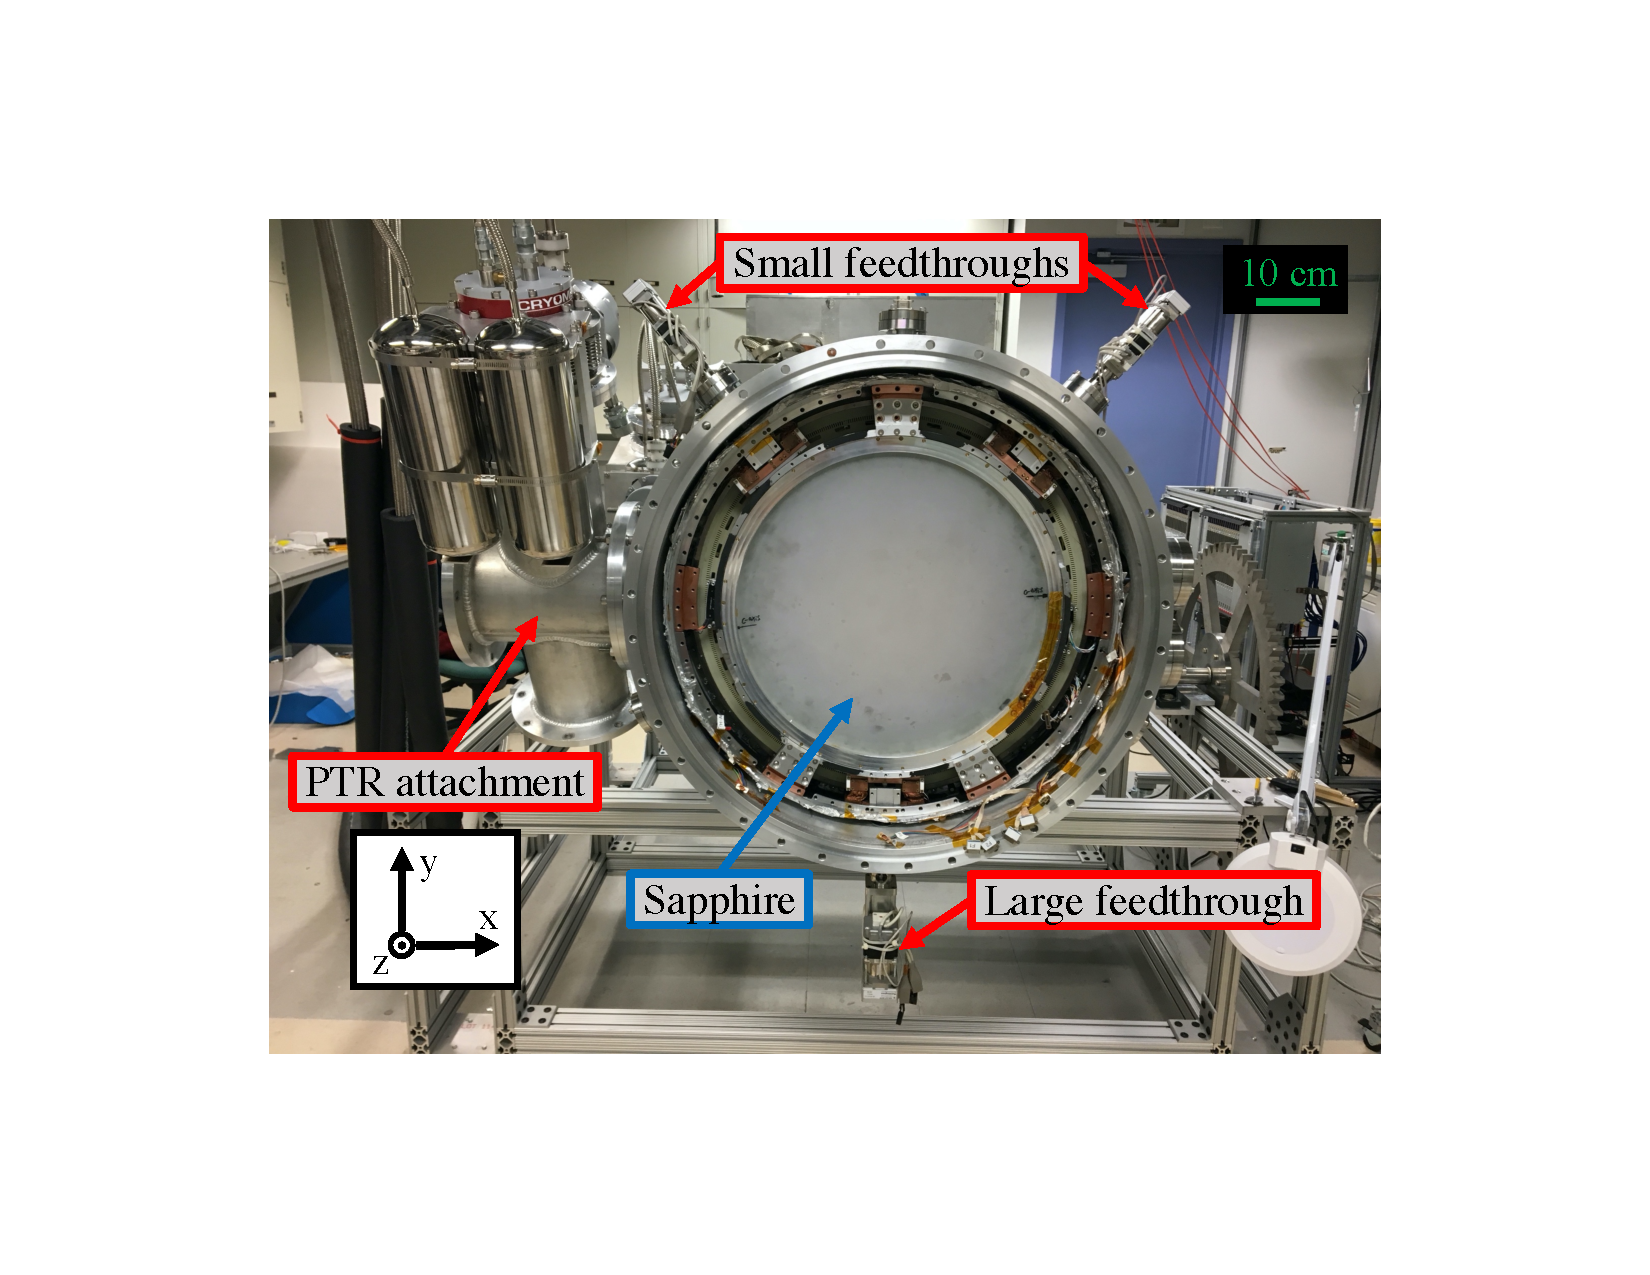
\includegraphics[width=0.7\linewidth, trim=4.4cm 4.5cm 4.5cm 3.5cm, clip]{CHWPEvaluation/Figures/CHWP_in_PB2b_photo.pdf}
    \caption{The CHWP mounted in the PB-2b receiver at UCSD. Before the gripper engages, the rotor is held by three installation stanchions that align it to the stator. The top two ``small'' gripper subassemblies are only separated by $80^{\circ}$ to avoid colliding with the PTR attachment. The single sapphire plate has no AR coating, and its frosty appearance is due to its $\sim \; 0.1 \; \mathrm{\mu m}$ RMS surface roughness.}
    \label{fig:chwp_in_pb2b}
\end{figure}

We divide a discussion of the CHWP evaluation into two subsections. First, we discuss operational testing, including spin-up, continuous rotation, thermal performance, and shutdown. Second, we present the CHWP's data quality and noise impact, including encoder jitter, magnetic interference, and rotor temperature stability.

%%%%%%%%%%%%%%%%%%%%%%%%%%%%%%%%
%%%%%%%%%%%%%%%%%%%%%%%%%%%%%%%%
%%%%%%%%%%%%%%%%%%%%%%%%%%%%%%%%

\section{Operational performance}
\label{sec:pb2b_chwp_operational_performance}

In this section, we review CHWP operation, focusing on the gripper, motor, bearing, and thermal performance. We evaluate the interfacing between various subsystems and show that the CHWP executes its essential functions while meeting the requirements shown in Table~\ref{tab:requirements}.

%%%%%%%%%%%%%%%%%%%%%%%%%%%%%%%%
%%%%%%%%%%%%%%%%%%%%%%%%%%%%%%%%

\subsection{Cooldown}
\label{sec:pb2a_chwp_evaluation_cooldown}

When the YBCO is above its $\approx$~90~K transition temperature, the gripper must keep the rotor centered, and between 300 and 50~K, the rotor contracts $\approx$~2~mm radially with respect to the vacuum shell. Therefore during cooldown, the gripper periodically ``re-grips'' the rotor, with each gripper finger inching inwards until the grip force is 50\% of the rotor's weight. This routine both keeps the rotor centered until the YBCO goes superconducting and maintains a conductive cooling path from the rotor to the stator baseplate. Figure~\ref{fig:gripper_cooldown} shows gripper-finger position vs. both rotor and stator temperature during an LBNL cooldown. In this particular test, the fingers are moved manually at convenient intervals, and their relative positions are maintained to <~0.2~mm, resulting in a rotor-stator coupling efficiency of $\approx$~99\% (see Figure~\ref{fig:motor_eff}). 

\begin{figure}[!t]
    \centering
    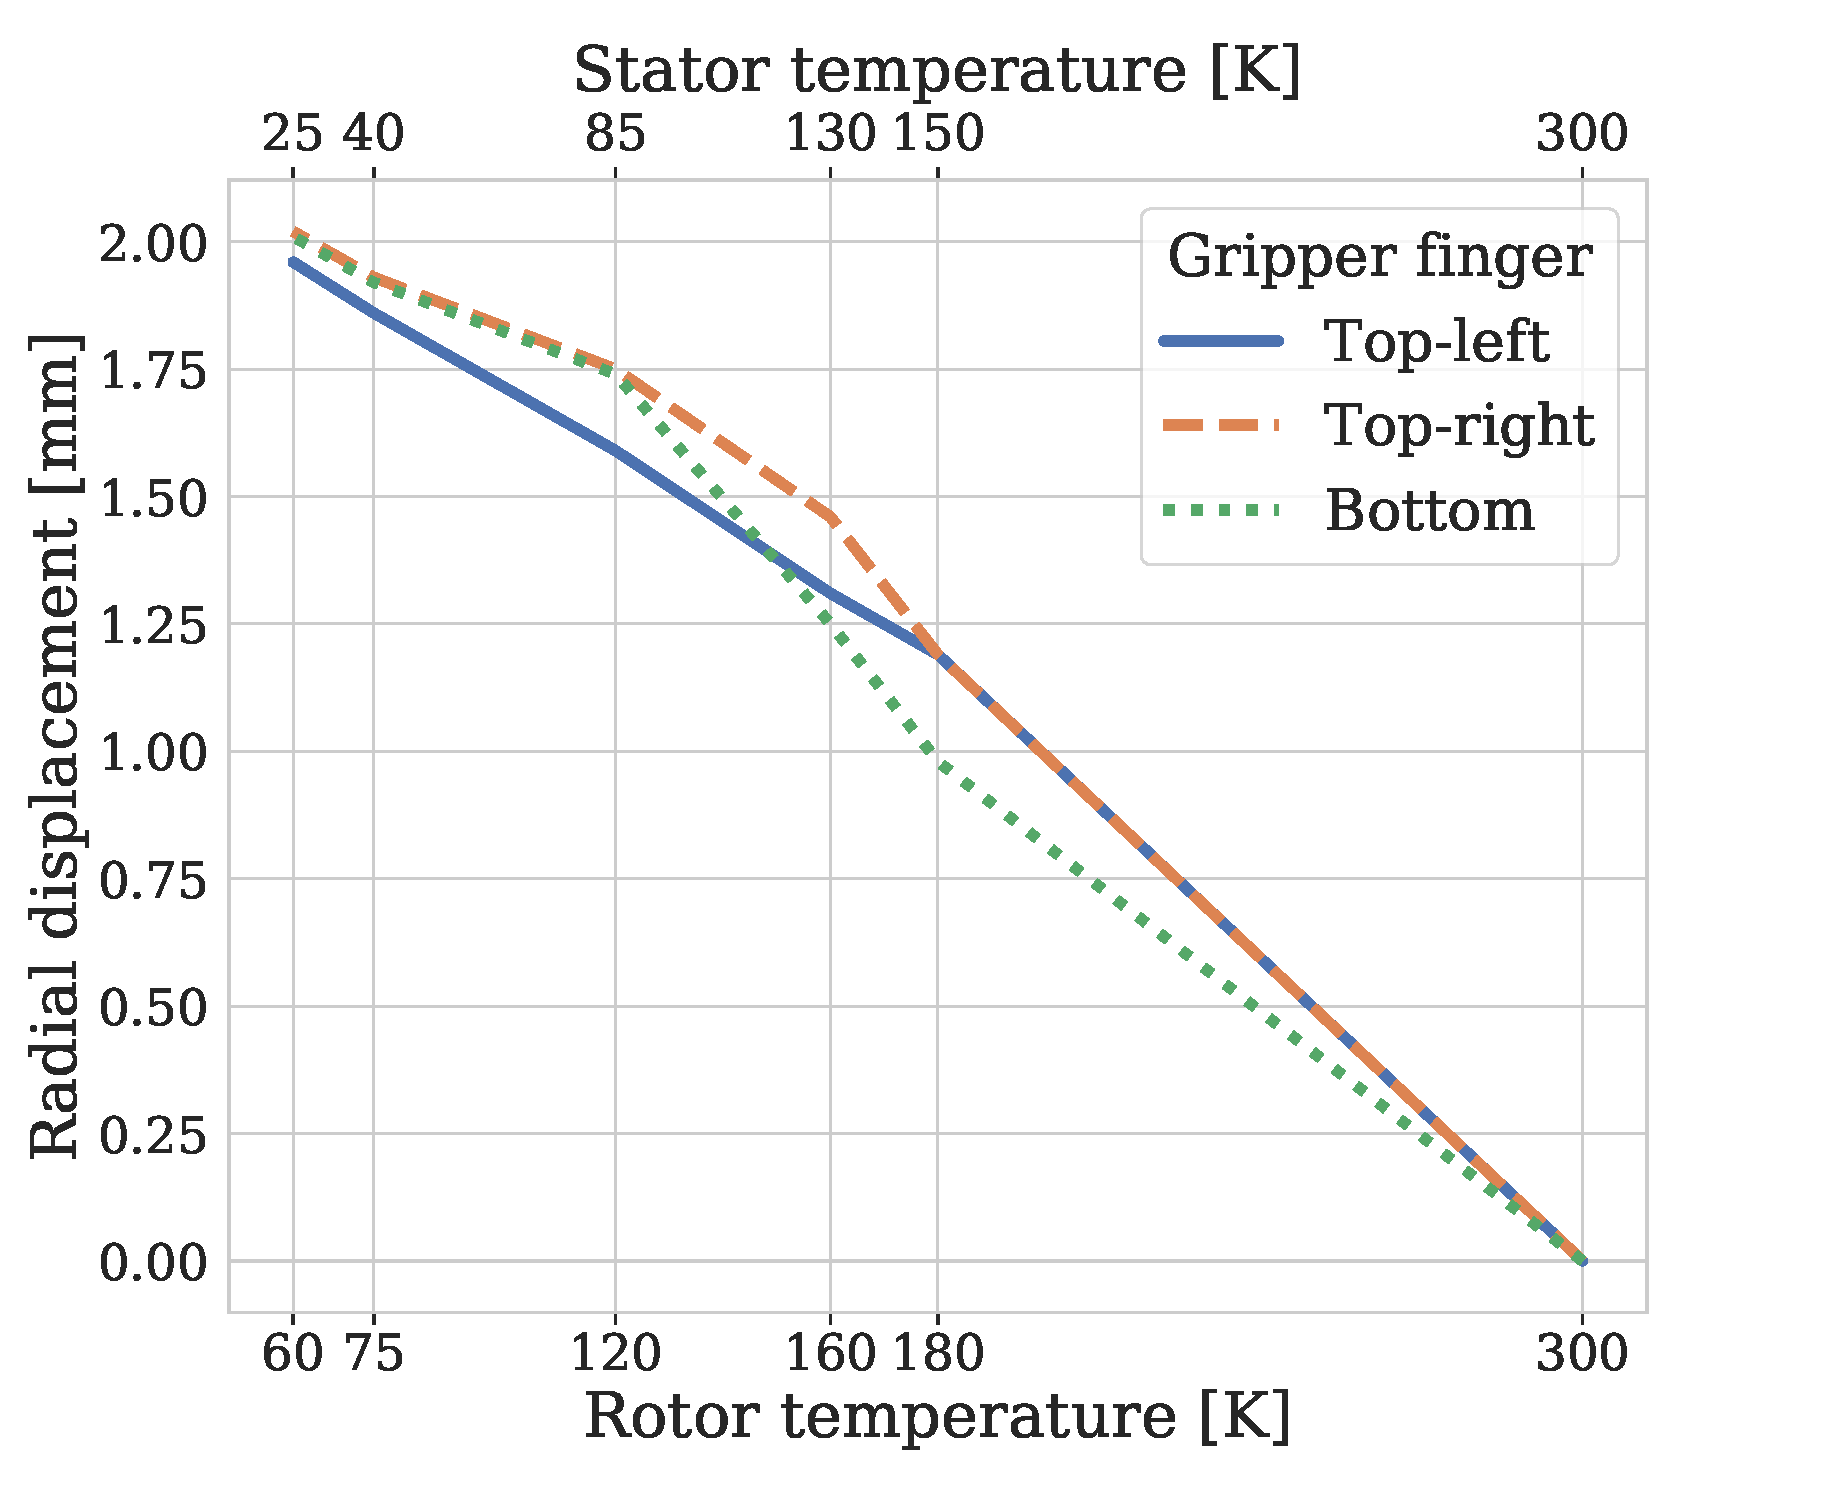
\includegraphics[width=0.6\linewidth, trim=0.5cm 0.9cm 2.8cm 0.7cm, clip]{CHWPEvaluation/Figures/gripper_cooldown.pdf}
    \caption{Radial displacement of each gripper finger vs. both rotor and stator temperature during LBNL testing. The gripper-finger labels refer to their locations in Figure~\ref{fig:chwp_in_pb2b}. The motors are manually commanded at convenient points during the $\approx$~100-hour cooldown, and their relative positions are maintained to $\leq$~0.2~mm throughout.}
    \label{fig:gripper_cooldown}
\end{figure}

Also during cooldown, the rotor's only cooling mechanisms are conduction through the gripper fingers and radiative coupling to the surrounding environment. Because the rotor's heat capacity is $\sim$~10~kJ/K at 300~K, good rotor-gripper contact conductance is needed for the CHWP to thermalize within 36 hours of the 50~K stage. The rotor stage's triangular groove and gripper fingers' triangular wedges are precision-cut to maximize thermal contact, and the measured rotor-to-gripper conductance is 0.7~W/K at 100~K. Figure~\ref{fig:rotor_cooldown} shows rotor and stator temperatures during a cooldown in the LBNL cryostat. The rotor lags behind the stator by only five~hours, which is well within the 36-hour requirement. 

\begin{figure}[!t]
    \centering
    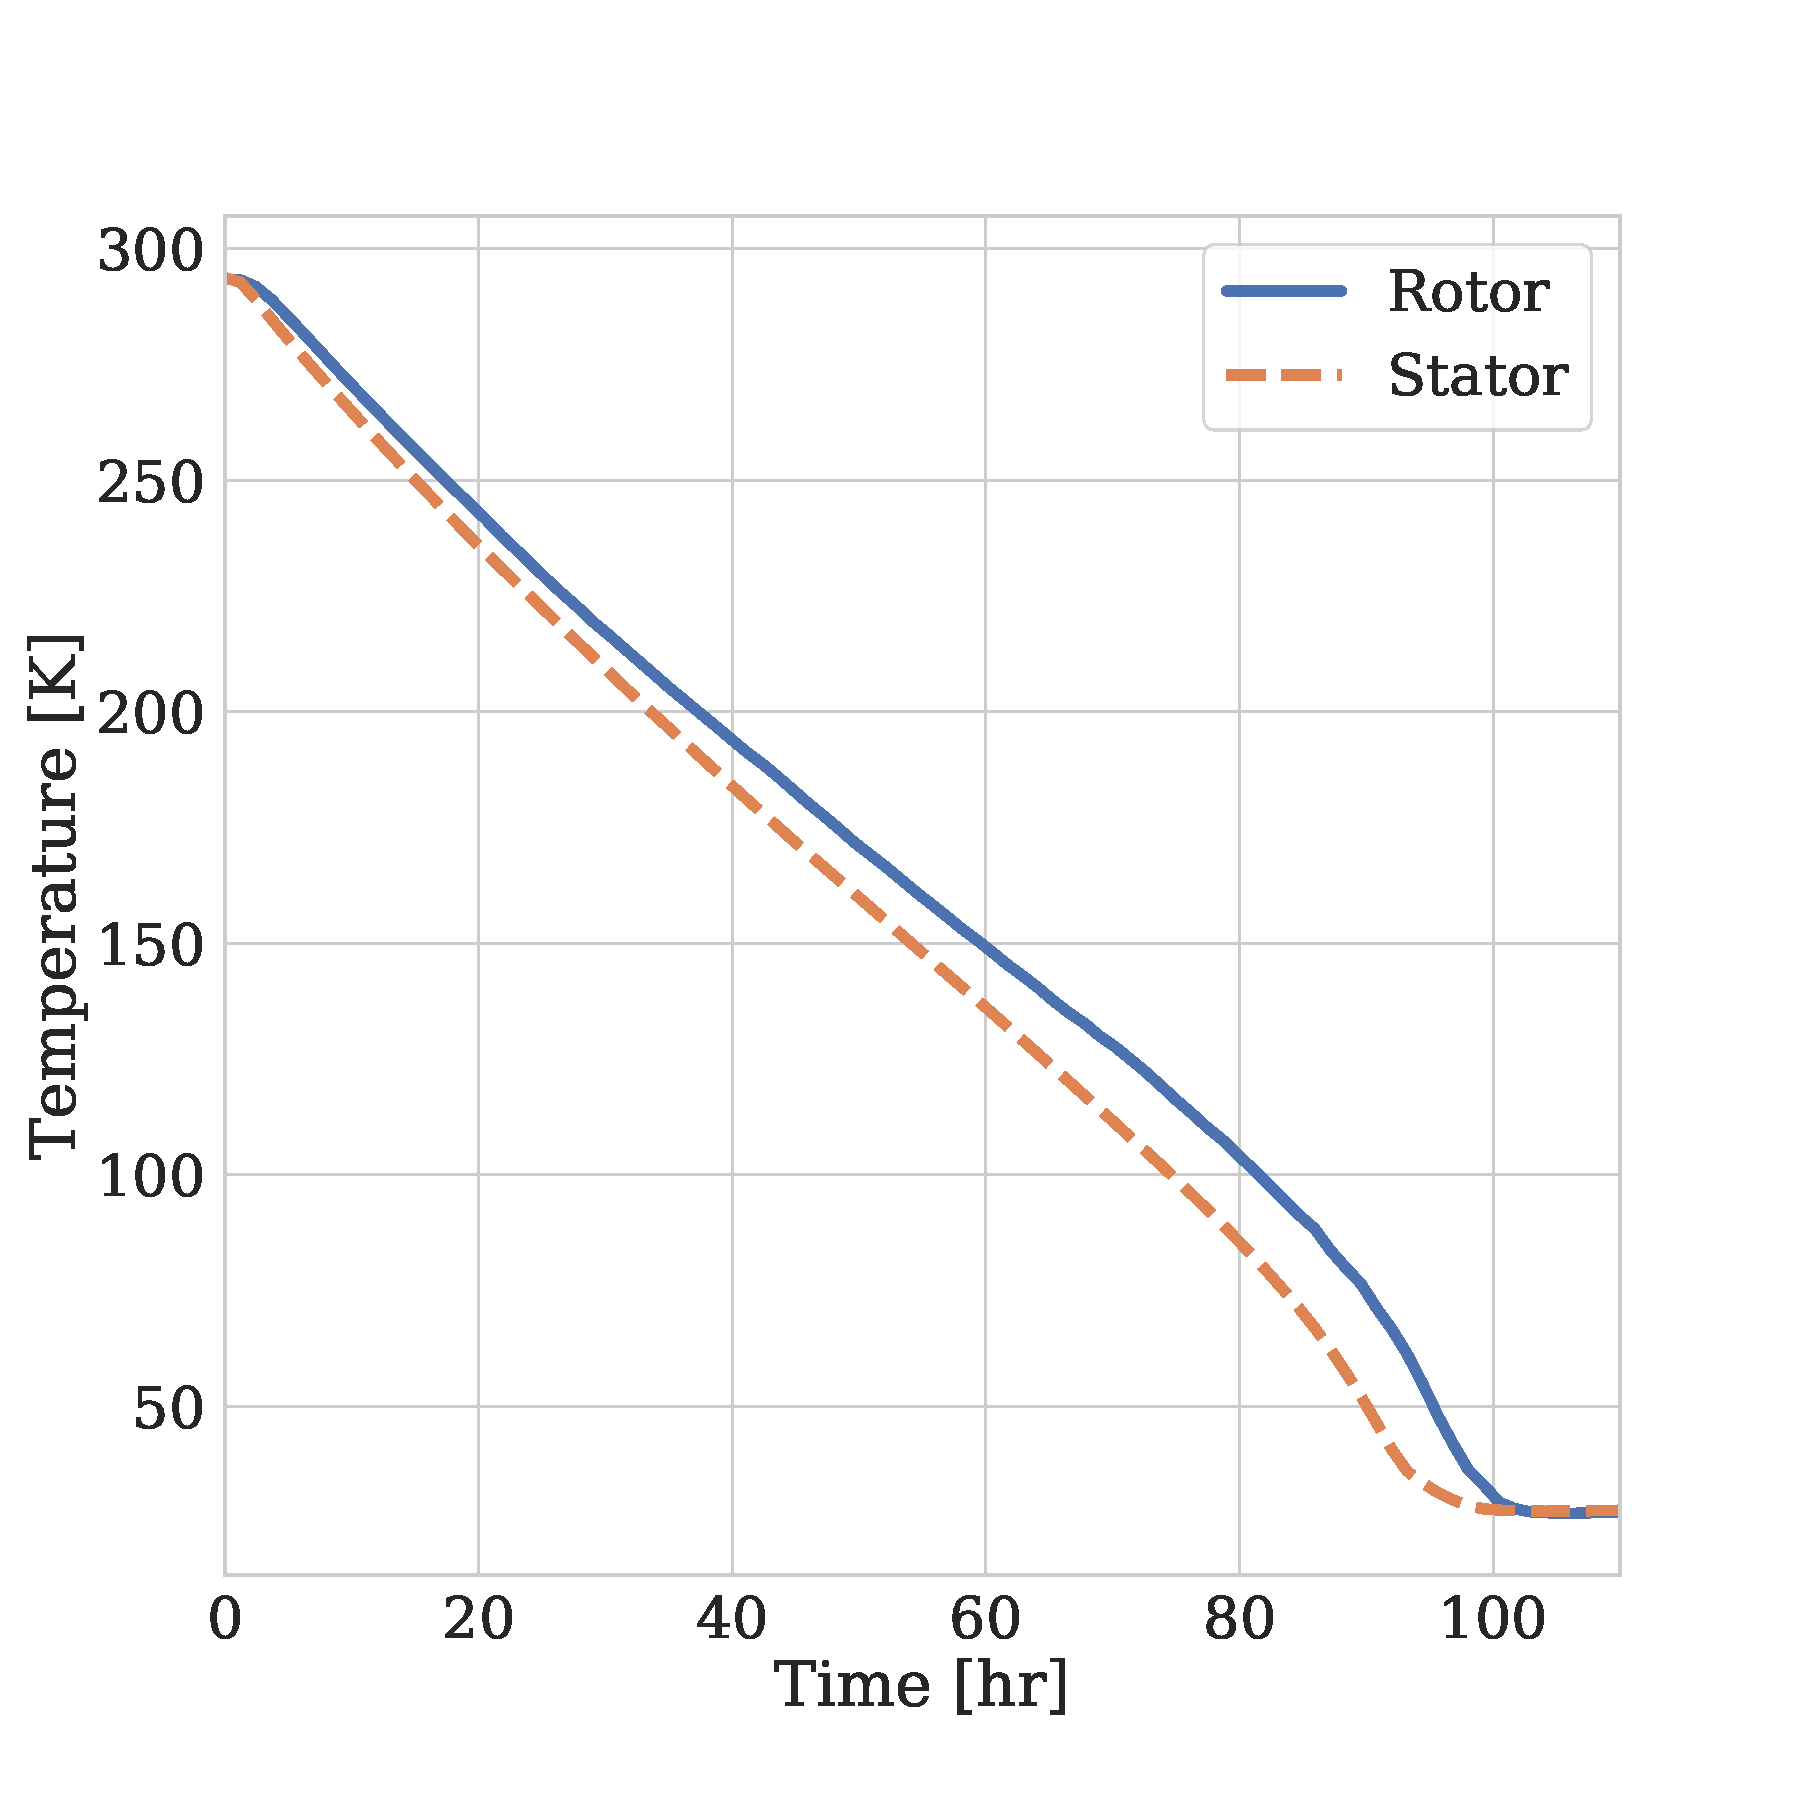
\includegraphics[width=0.6\linewidth, trim=0.5cm 1cm 2.5cm 2.4cm, clip]{CHWPEvaluation/Figures/chwp_cooldown.pdf}
    \caption{CHWP temperatures during a cooldown to 25 K in the LBNL dark cryostat. While the rotor lags behind the stator by $\approx$~10~K, it thermalizes within five hours of its surroundings.}
    \label{fig:rotor_cooldown}
\end{figure}

%%%%%%%%%%%%%%%%%%%%%%%%%%%%%%%%
%%%%%%%%%%%%%%%%%%%%%%%%%%%%%%%%

\subsection{Start-up}
\label{sec:pb2a_chwp_evaluation_start_up}

After the YBCO becomes superconducting and the CHWP assembly thermalizes, the rotor is held in place for a few hours to let the bearing ``relax.'' Flux pinning needs time to find its lowest-energy configuration \cite{postrekhin_dynamics_2001}, and if the rotor moves during this relaxation, pinning sites are more likely to escape the superconducting bulk, hence reducing the bearing's spring constant. This flux migration is logarithmic in time, with the vast majority of equilibration occurring within hours of the YBCO transition. After the bearing has relaxed, the gripper fingers retract and the stator supports the rotor's weight. When the receiver is horizontal, as in Figure~\ref{fig:chwp_in_pb2b}, the rotor is observed to ``sag'' away from its gripped position by 0.5~mm, and because the bearing's spring force is elastic, this displacement decreases with increasing receiver inclination.

When floating and stationary, forces between the magnet sprockets and the solenoids' ferromagnetic cores keep the rotor azimuthally constrained. In order to overcome this stiction during start-up, the motor energizes with $\approx$~0.4~A (or $\sim$~5$\times$ its current draw during continuous operation). Once rotation commences, cogging quickly diminishes, the rotor transitions into smooth rotation, and the solenoid bias is reduced. Rotation frequency vs. time for various H-driver voltages during spin-up are shown in Figure~\ref{fig:spin_up}. The achievable rotation frequencies are 1.8-2.8~Hz, and the equilibration time is tens of minutes. While PID control will reduce the start-up time somewhat, the CHWP is intended to run without interruption throughout each day's telescope observations, and therefore this level of latency meets PB-2b's needs.

\begin{figure}[!t]
    \centering
    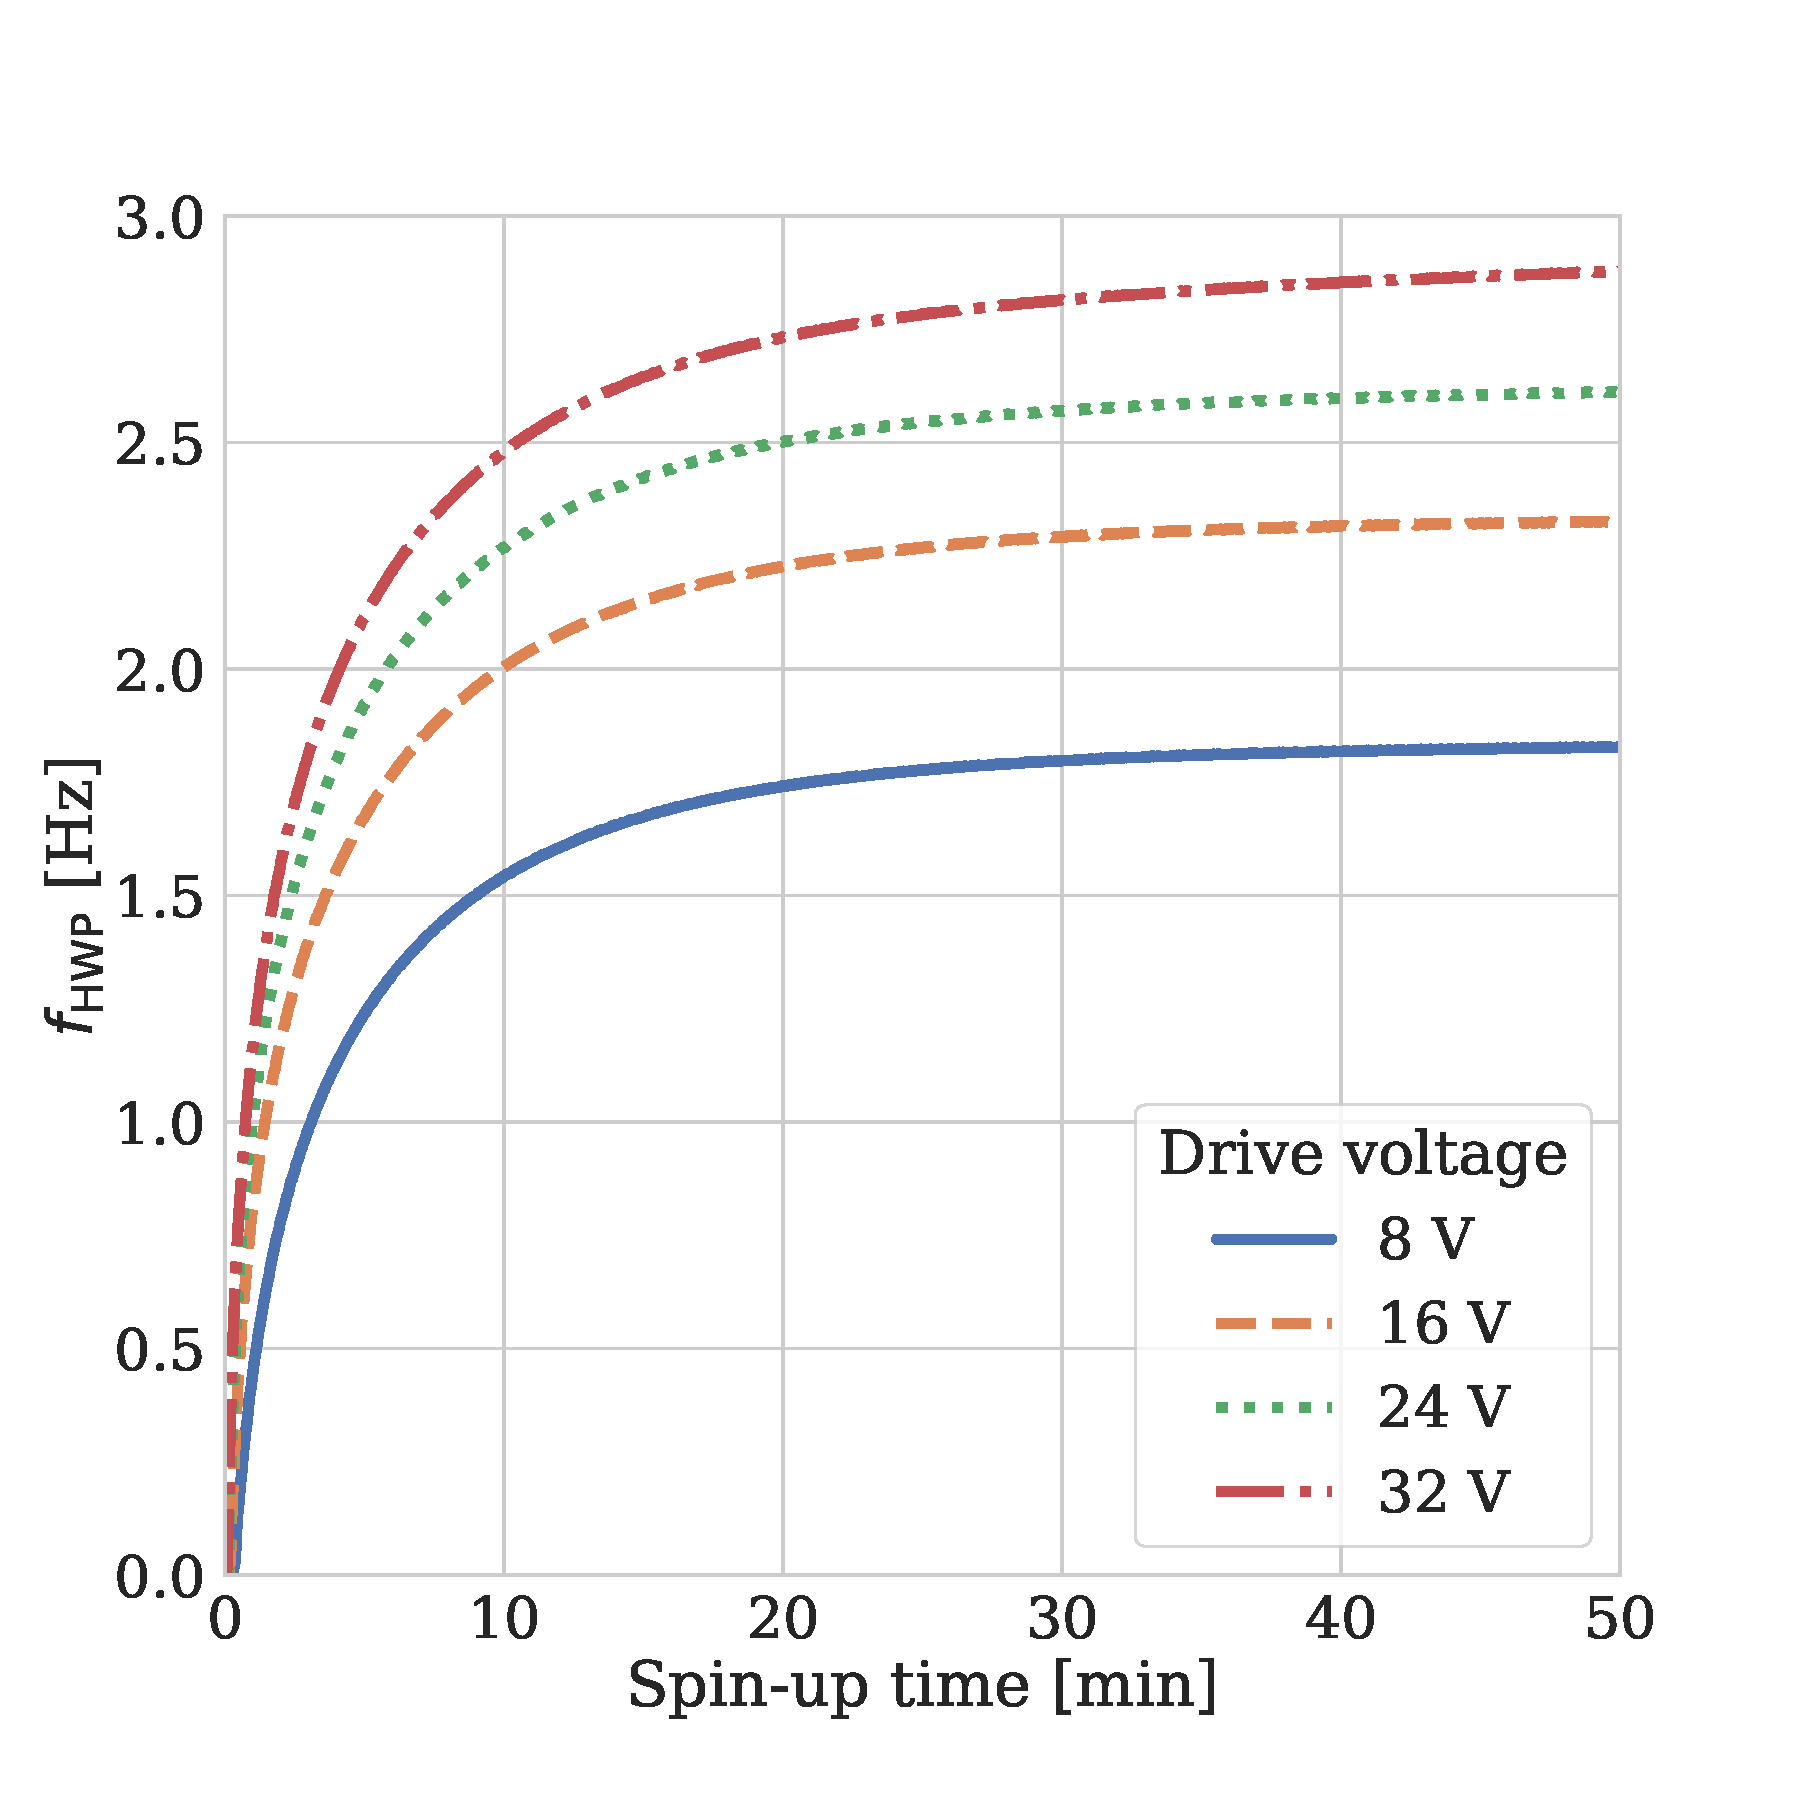
\includegraphics[width=0.6\linewidth, trim=0.5cm 1.2cm 2.5cm 3cm, clip]{CHWPEvaluation/Figures/rotor_spinup.pdf}
    \caption{CHWP rotation frequency vs. time during start-up for various H-driver voltages in the LBNL cryostat. The motor attains rotation frequencies up to $\approx$ 2.8 Hz, at which point it becomes limited by motor-phase-delay efficiency (see Figure~\ref{fig:motor_eff}) and rotor friction (see Figure~\ref{fig:rot_pow_diss}).}
    \label{fig:spin_up}
\end{figure}

%%%%%%%%%%%%%%%%%%%%%%%%%%%%%%%%
%%%%%%%%%%%%%%%%%%%%%%%%%%%%%%%%

\subsection{Continuous rotation}
\label{sec:pb2a_chwp_evaluation_continuous_rotation}

Once spun up, the CHWP enters constant velocity mode. To measure the CHWP's open-loop stability, we collect one hour of continuous rotation data in the LBNL test cryostat without PID control. Such a test helps identify any pathologies in the drive system that may manifest as modulations in rotational velocity. While the PB-2b CHWP does not have a velocity stability requirement, steady rotation helps assess encoding accuracy, which is discussed in Section~\ref{sec:pb2b_chwp_evaluation_encoder_jitter}.

Figure~\ref{fig:rot_stability} shows velocity drift vs. time at $f_{\mathrm{HWP}} = 2.15 \; \mathrm{Hz}$. The total $\Delta f_{\mathrm{HWP}}= 0.8$~mHz corresponds to a rotational stability of 0.04\%/hr, which is much better than that of ABS \cite{kusaka_modulation_2014} and PB-1. While changes in telescope inclination will slightly modulate rotor-stator concentricity, which in turn modulates motor efficiency (see Section~\ref{sec:motor_eff}), we anticipate even better stability when using PID control in the field (see Section~\ref{sec:motor_design}).

\begin{figure}[!t]
    \centering
    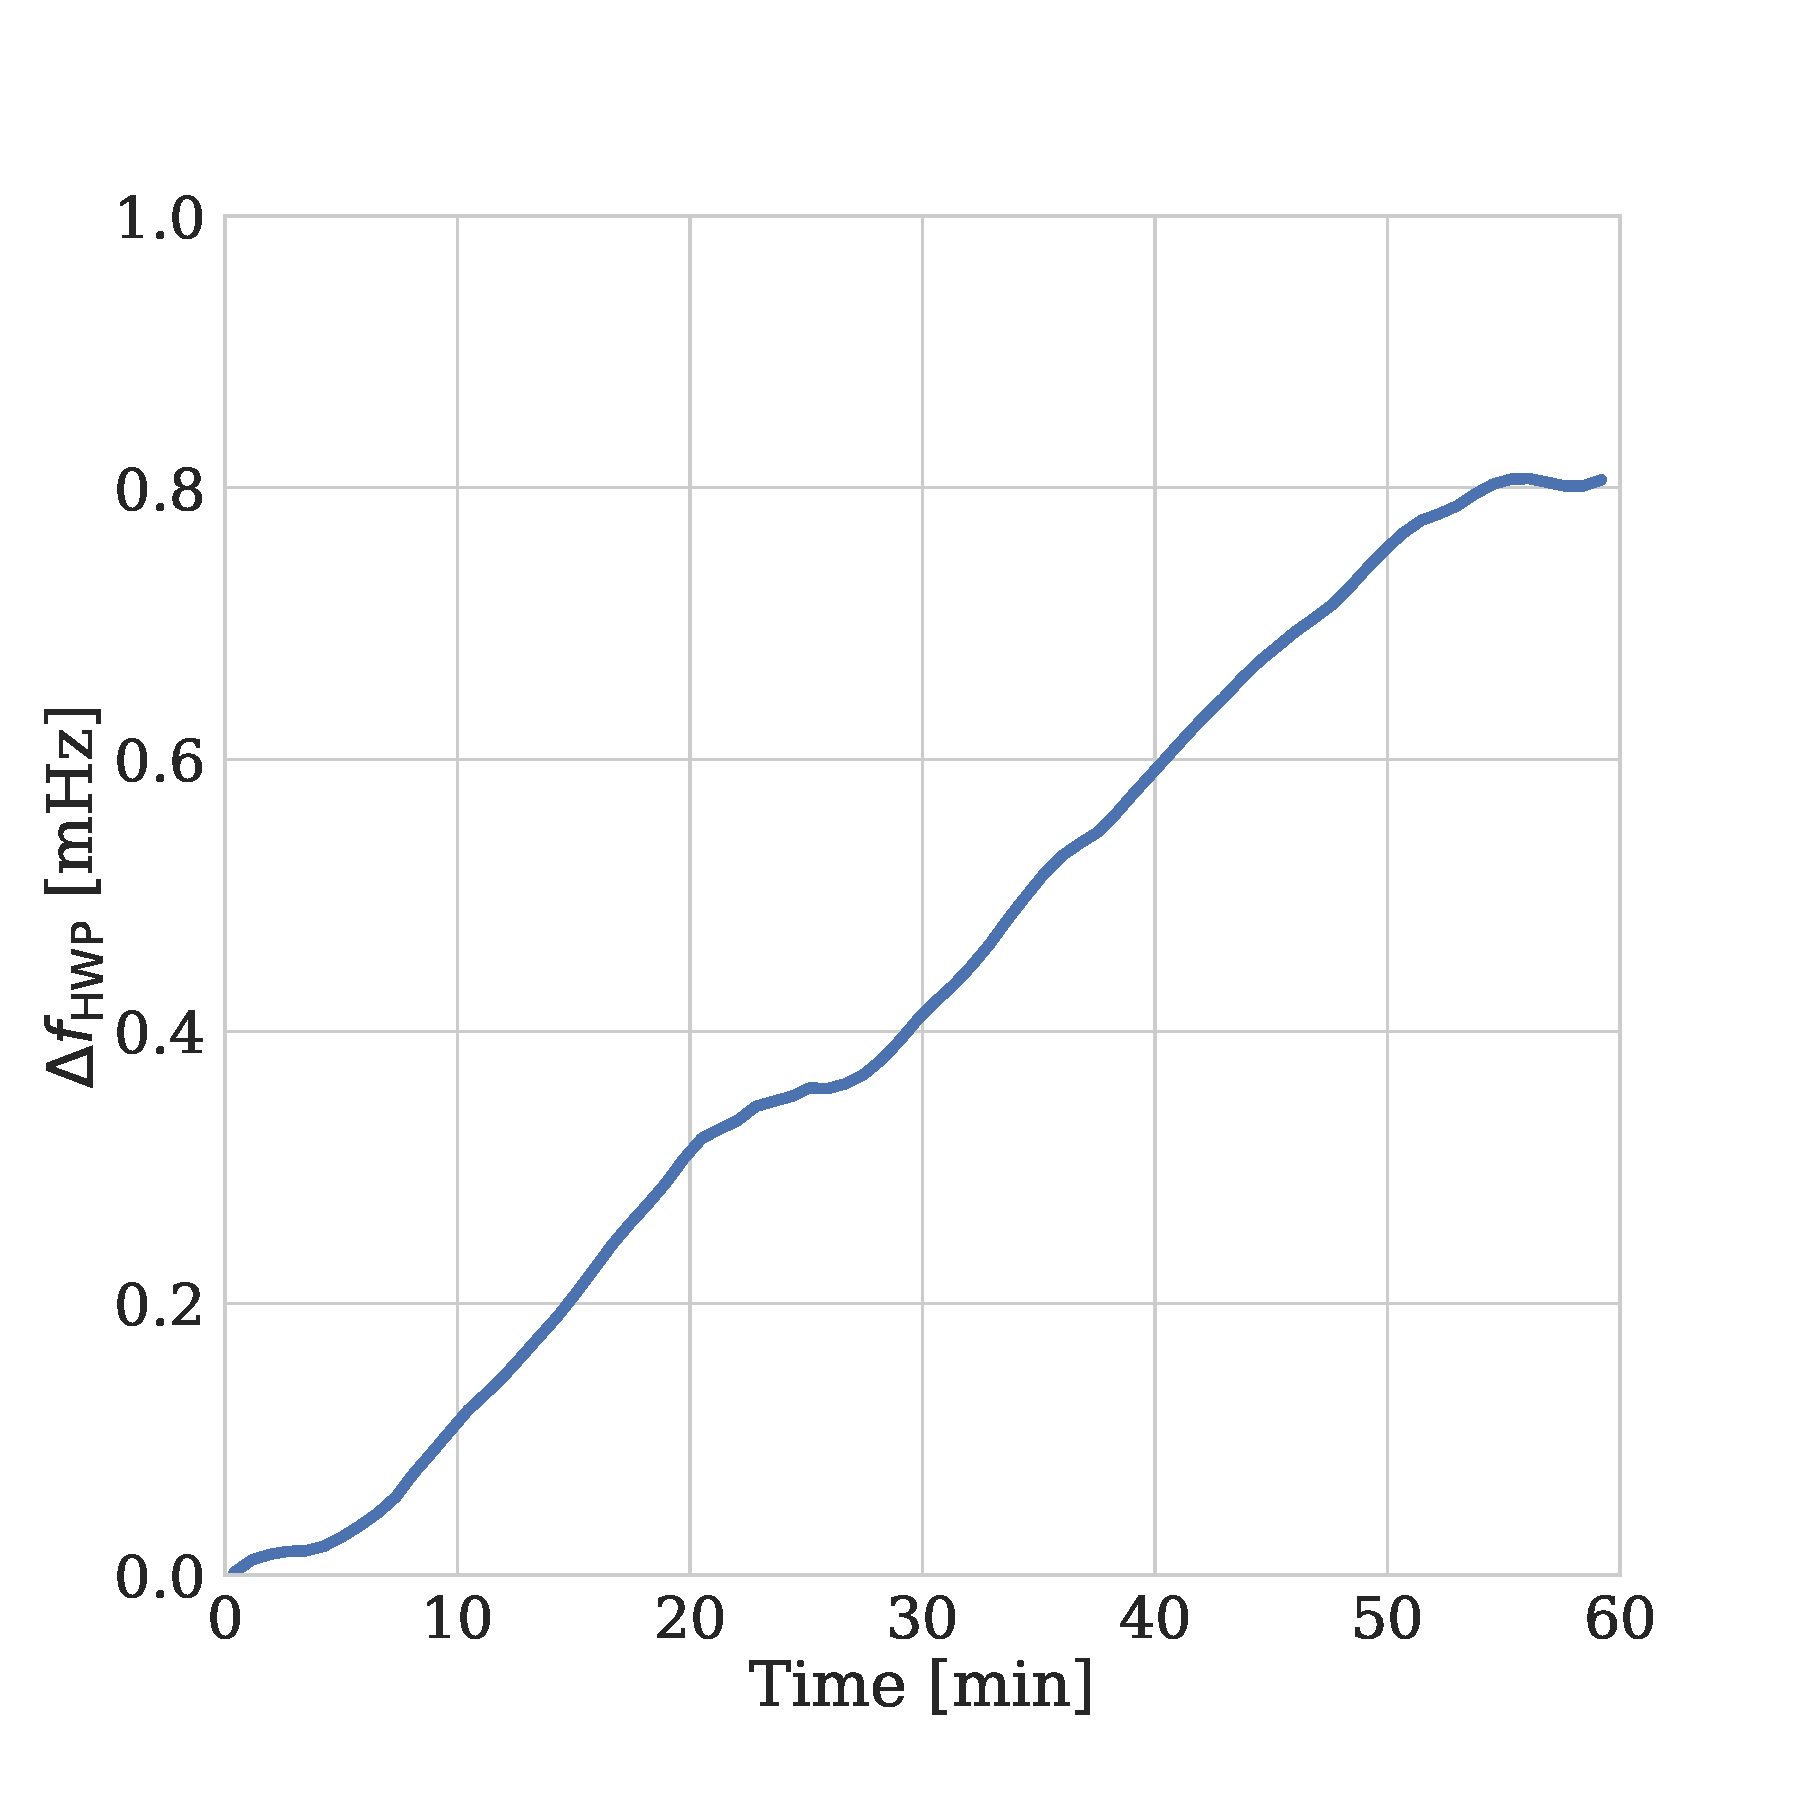
\includegraphics[width=0.6\linewidth, trim=0.5cm 1.4cm 2.5cm 3cm, clip]{CHWPEvaluation/Figures/velocity.pdf}
    \caption{$\Delta f_{\mathrm{HWP}}$ during one hour of continuous rotation in the LBNL cryostat, sampled once per rotation and averaged over one-minute intervals. The mean velocity is $f_{\mathrm{HWP}} = 2.15$~Hz, and therefore the fractional stability is 0.04\%/hr.}
    \label{fig:rot_stability}
\end{figure}

\begin{figure}
    \subfloat[\label{fig:chwp_magnetic_noise:a}]{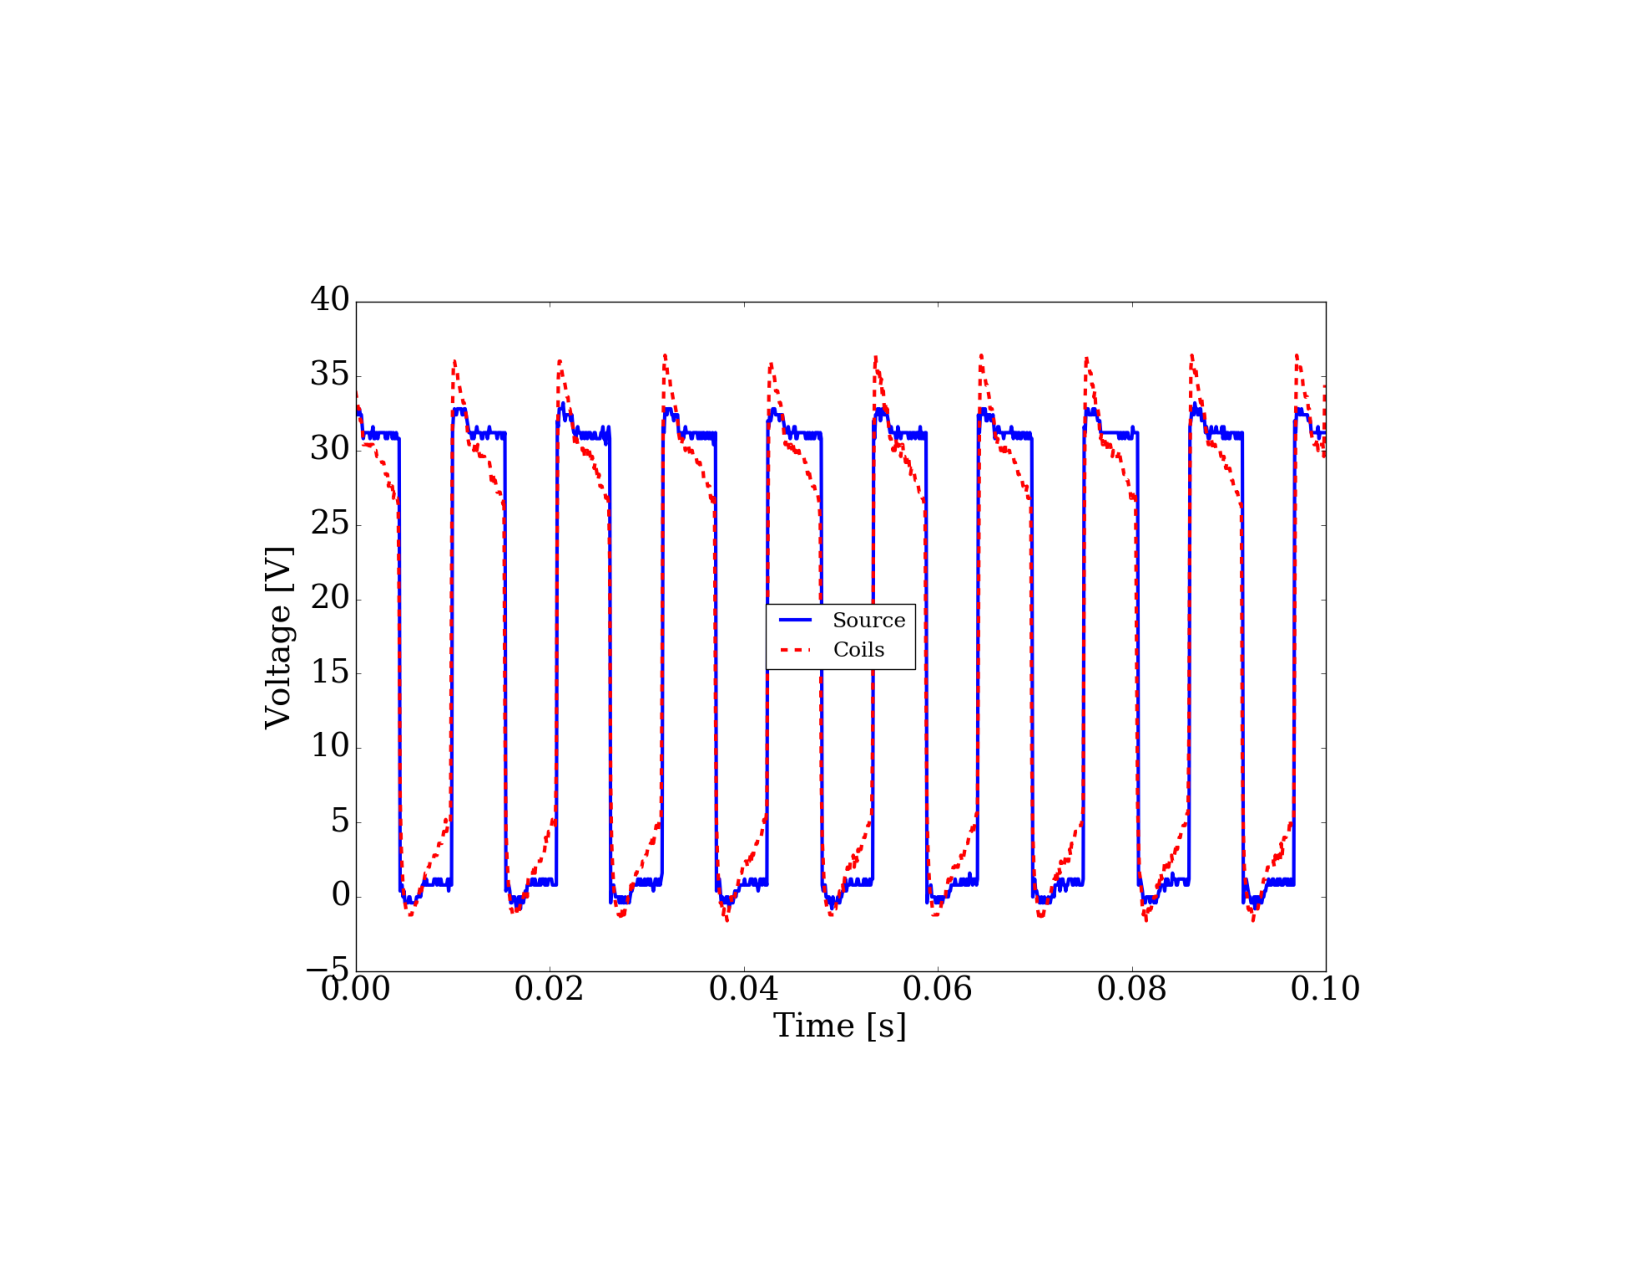
\includegraphics[width=0.48\linewidth, trim=3.9cm 3.8cm 5cm 4.5cm, clip]{CHWPEvaluation/Figures/chwp_motor_waveform.pdf}}
    \subfloat[\label{fig:chwp_magnetic_noise:b}]{
        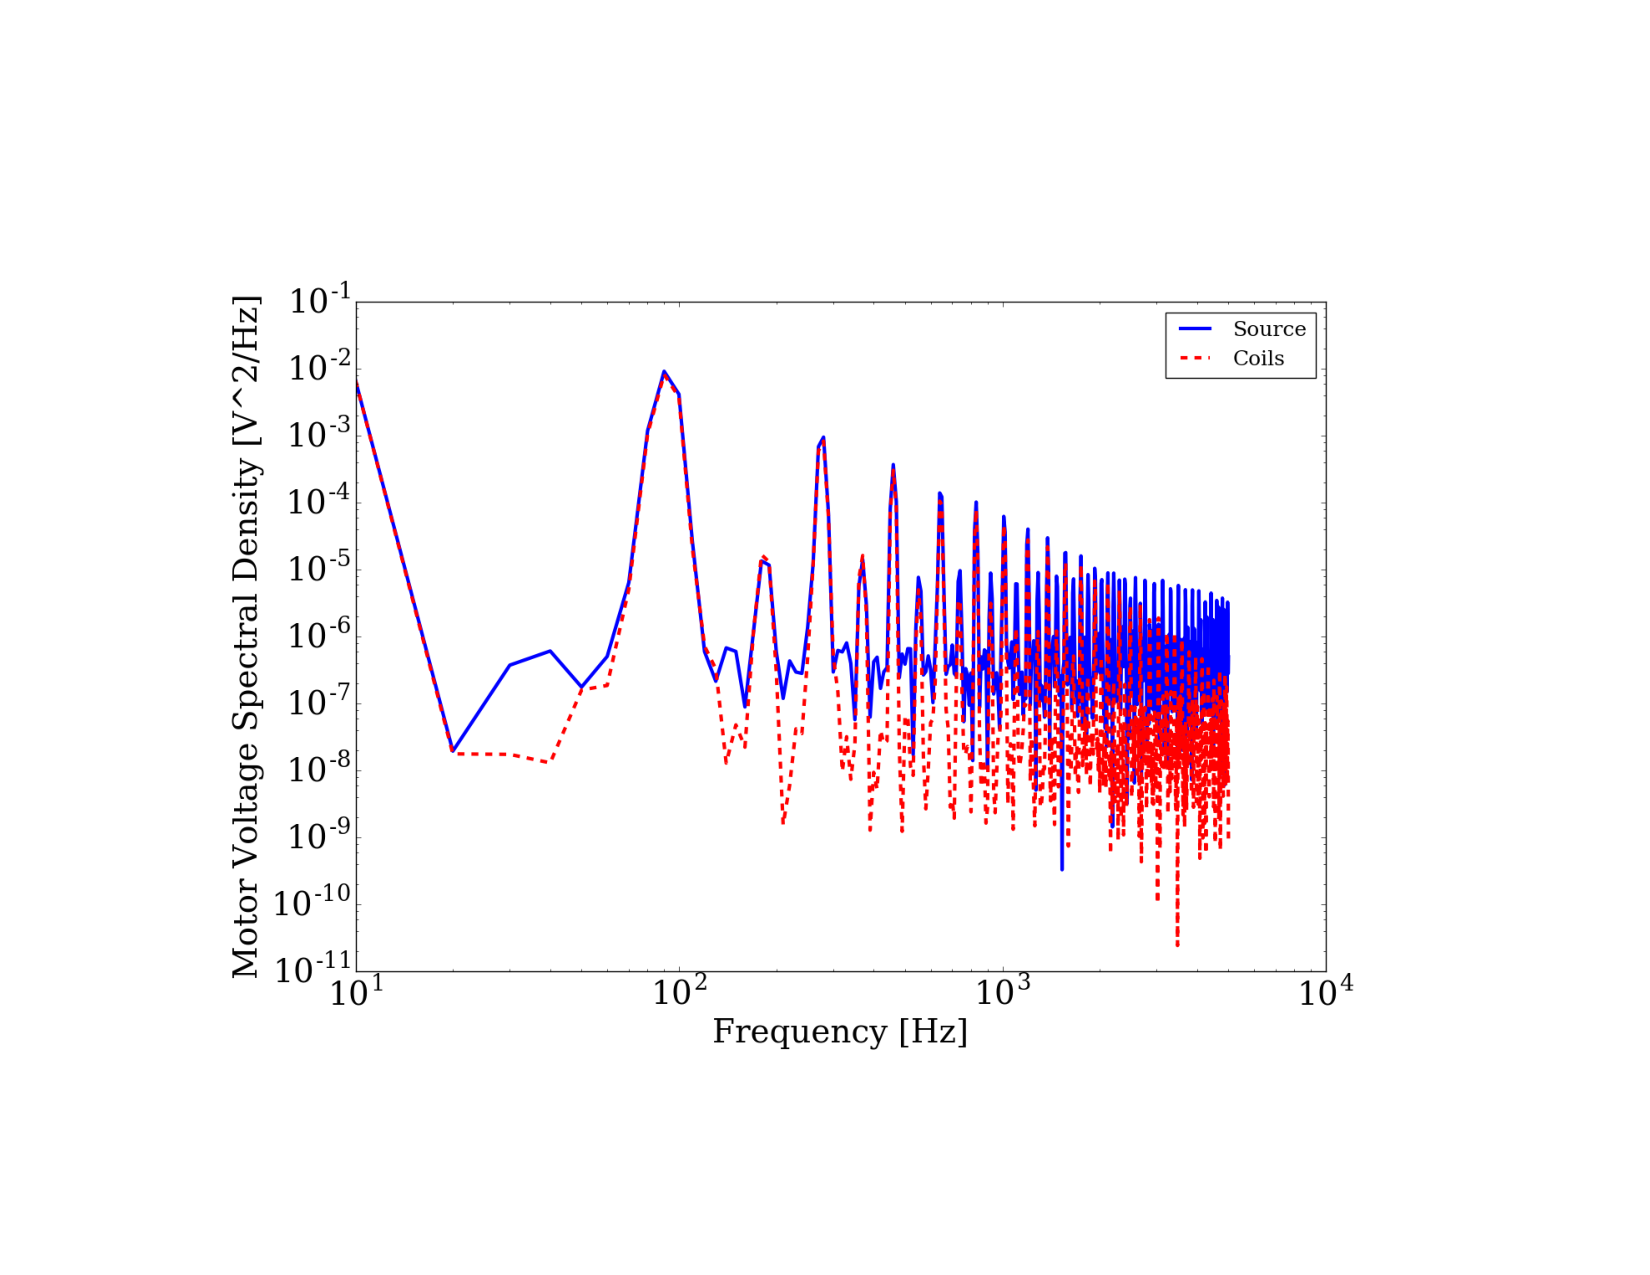
\includegraphics[width=0.48\linewidth, trim=3.5cm 3.8cm 5.3cm 4cm, clip]{CHWPEvaluation/Figures/chwp_motor_psd.pdf}}
    \caption[CHWP motor waveforms and power spectral densities. ]{CHWP motor waveforms and power spectral densities when driving at 32~V and a rotation frequency of $f_{HWP} \approx 3$~Hz. Figure~\ref{fig:chwp_magnetic_noise:a} shows an output waveform from a motor H-driver. The blue line shows the voltage output at the driver IC, and the red dotted line shows the voltage across the motor solenoids. The conversion from a rectangular to a triangular waveform shape is due to the low-pass filter, and the rising-edge peaks are inductance voltage spikes across the motor solenoids. Figure~\ref{fig:chwp_magnetic_noise:b} shows the power spectral density of the motor voltage waveform. The peaks correspond to the motor frequency of $\approx$~100~Hz, and the power roll-off demonstrates the low-pass filter's $\approx$~300~Hz -3~dB frequency.}
    \label{fig:chwp_magnetic_noise}
\end{figure}

%%%%%%%%%%%%%%%%%%%%%%%%%%%%%%%%
%%%%%%%%%%%%%%%%%%%%%%%%%%%%%%%%

\subsection{Thermal impact}
\label{sec:pb2a_chwp_evaluation_thermal_impact}

The CHWP's thermal impact is evaluated in three stages. First, we measure rotor friction and motor dissipation in the LBNL cryostat. Rotor friction is determined by measuring deceleration vs. velocity with the motor powered off, and motor dissipation is determined by measuring the current through and resistance of the solenoids. Dissipation as a function of rotation frequency is shown in Figure~\ref{fig:rot_pow_diss}, and at 2~Hz, rotor and motor heating are 80~mW and <~200~mW, respectively. A polynomial fit to rotor dissipation vs. $f_{\mathrm{HWP}}$ shows that at 2~Hz, most friction is due to eddy currents ($P_{\mathrm{eddy}} \propto f_{\mathrm{HWP}}^{2}$) as opposed to hysteresis loss ($P_{\mathrm{hyst}} \propto f_{\mathrm{HWP}}$). The motor dissipation data points represent measured values with excellent alignment at $T_{\mathrm{rotor}} = 60$~K, and the bands quantify possible variations in motor torque due to variations in rotor-stator concentricity and solenoid temperature. The motor dissipation's steep slope is due to both decreasing motor efficiency and increasing rotor friction with increasing $f_{\mathrm{HWP}}$.

\begin{figure}[!t]
    \centering
    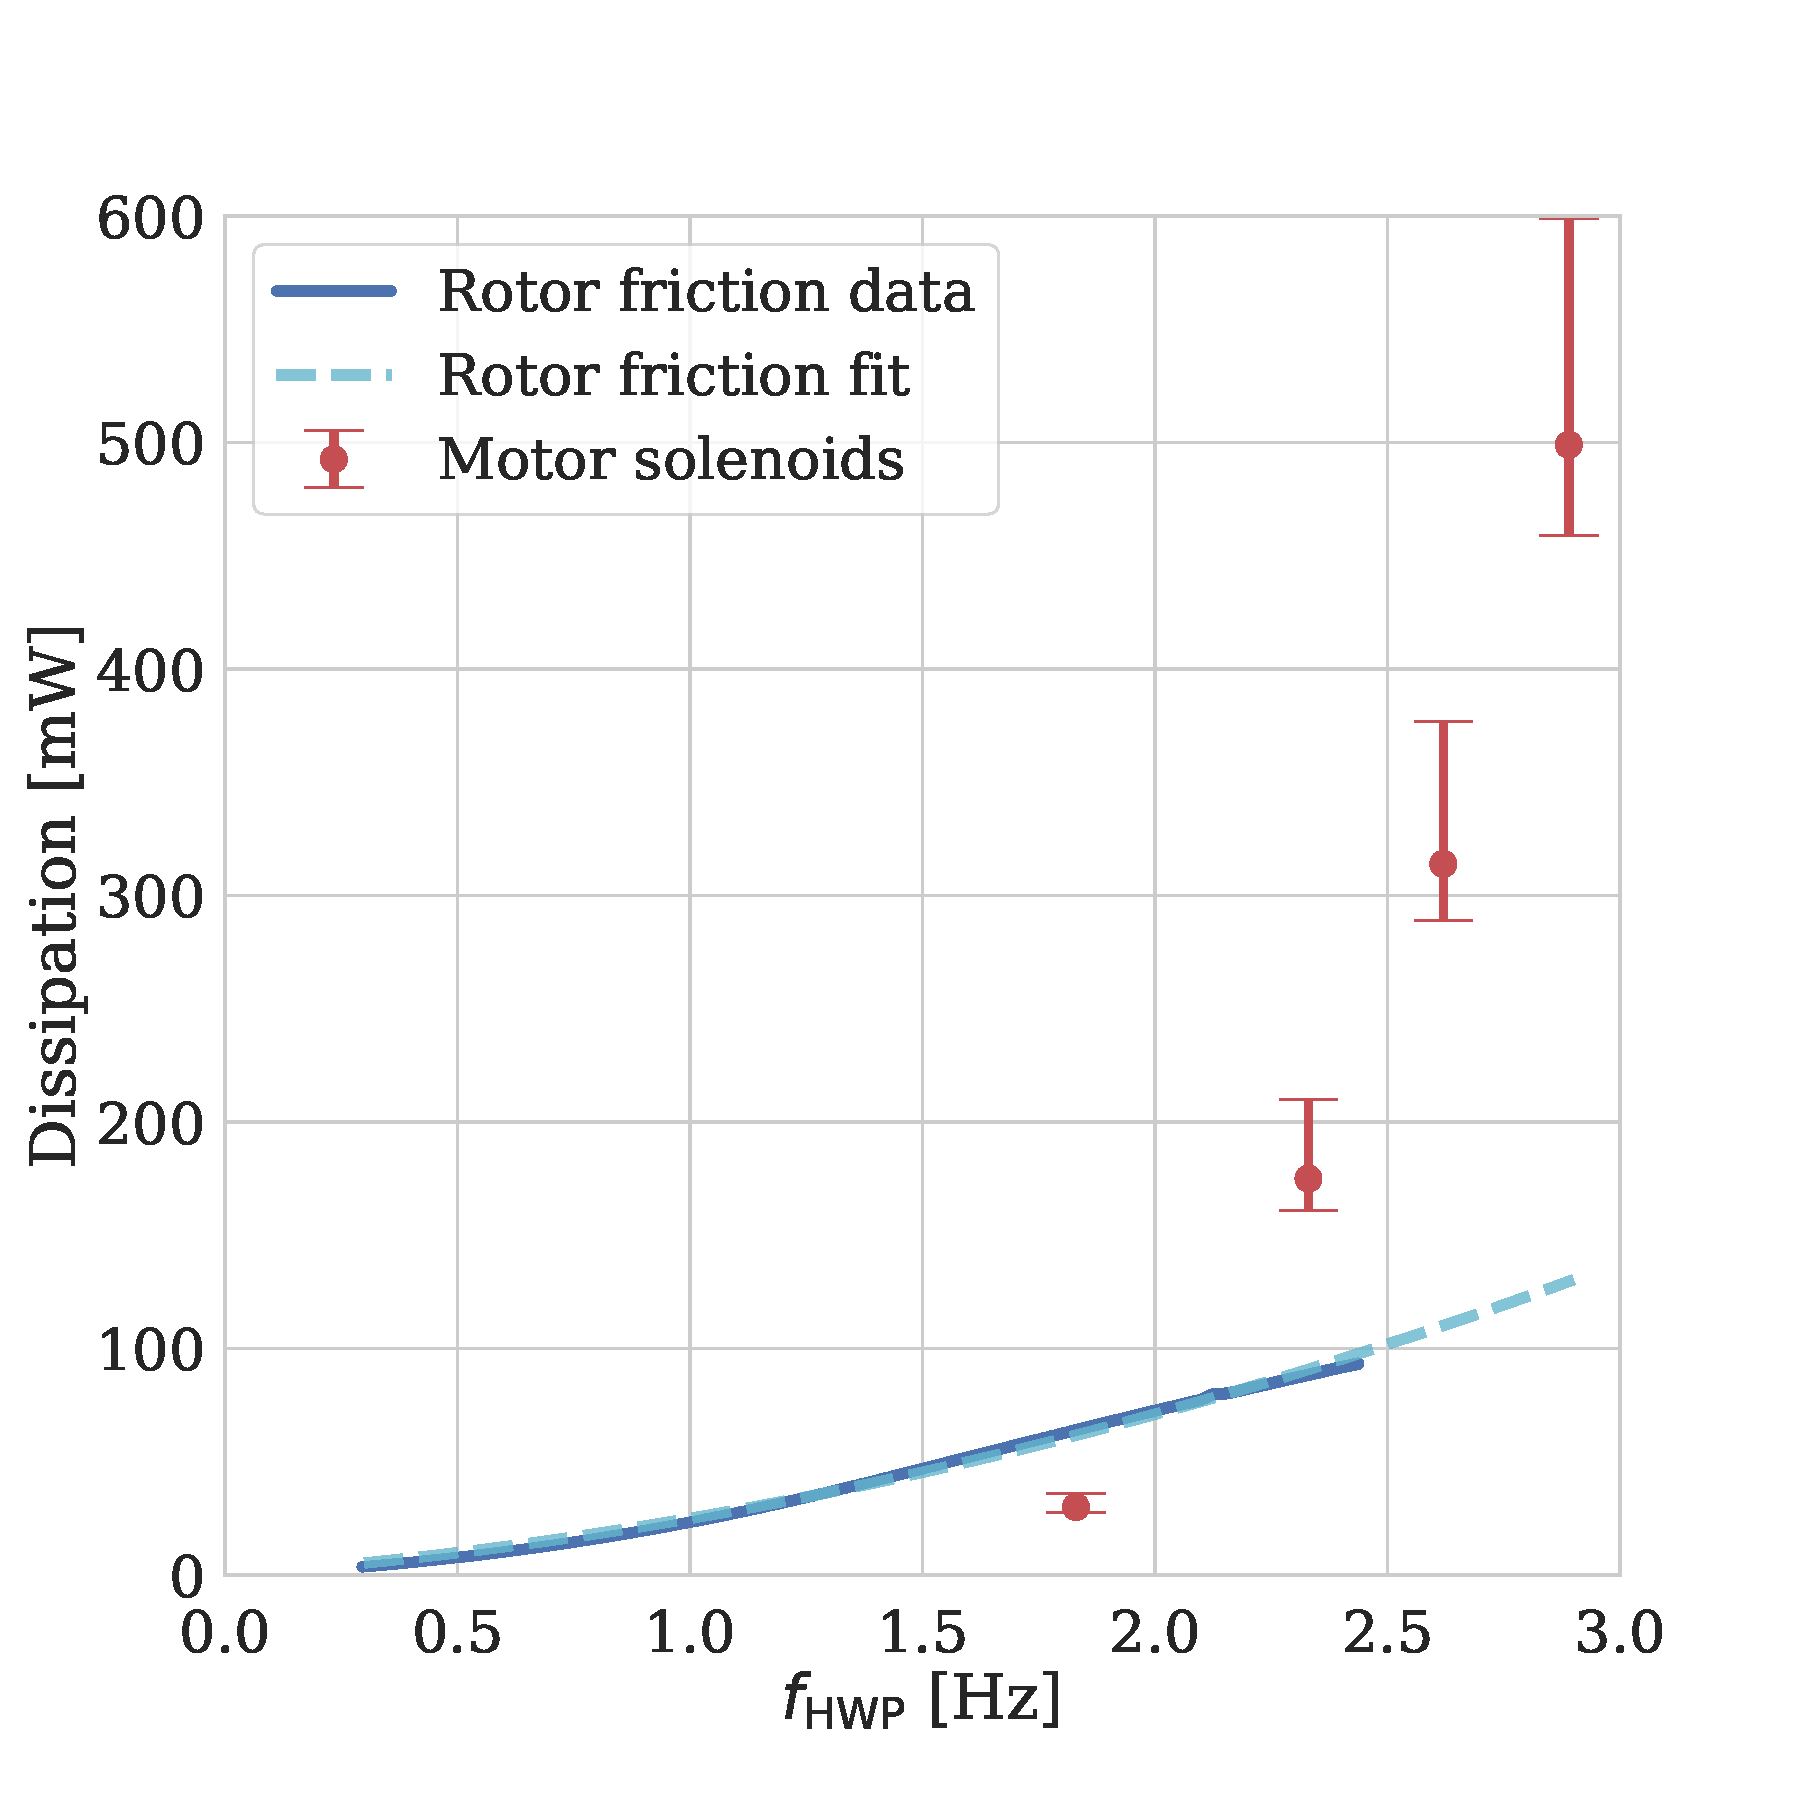
\includegraphics[width=0.6\linewidth, trim=0.4cm 1.2cm 2.3cm 3.2cm, clip]{CHWPEvaluation/Figures/rotor_motor_dissipation.pdf}
    \caption{Measured $f_{\mathrm{HWP}}$-dependent dissipation during continuous rotation. As described in Section~\ref{sec:pb2a_chwp_evaluation_thermal_impact}, a polynomial fit shows that rotor friction at 2~Hz is predominantly due to eddy-current losses, while motor dissipation is due to resistive heating in the solenoid array. The motor dissipation's error bars represent possible variations due to rotor positioning, solenoid temperature, and cryostat angle.}
    \label{fig:rot_pow_diss}
\end{figure}

Second, we evaluate cryo-optical performance in the UCSD test setup shown in Figure~\ref{fig:chwp_in_pb2b}. Even though this configuration has no AR coatings on the IRF, sapphire stack, or lenses, bare alumina and sapphire are largely IR absorptive, allowing us to evaluate the thermal model presented in Section~\ref{sec:thermal_design}. During UCSD testing, the CHWP's rotor thermometer disconnected, leaving us to infer the rotor's temperature rather than monitor it directly. Using a load curve of the field lens \cite{howe_polarbear-2_2019} and comparing field-lens and 50~K temperatures to a dark run without the CHWP \cite{howe_polarbear-2_2019}, we measure a rotor temperature of $<$~50~K and a field-lens temperature of 6.4~K, both of which are $\approx$~1$\sigma$ better than the thermal model's expectation after accounting for no AR coatings.\footnote{With one piece of 3.8~mm thick sapphire and with no AR coatings, the rotor temperature and field-lens power in the UCSD test are expected to be lower and higher, respectively, than shown in Figure~\ref{fig:rotor_temp}.} On the other hand, we measure a 50~K load of $\approx$~2.5~W, which is larger than the 2~W requirement. This test was performed before adopting the solenoid heat sinking scheme described in Section~\ref{sec:thermal_design}, which has been shown to reduce solenoid heating by $\sim$ 5x in auxiliary tests. Therefore, we anticipate a stator load consistent with the thermal model's $<$~1.3~W expectation when the CHWP operates in Chile.

\begin{figure}[!t]
    \centering
    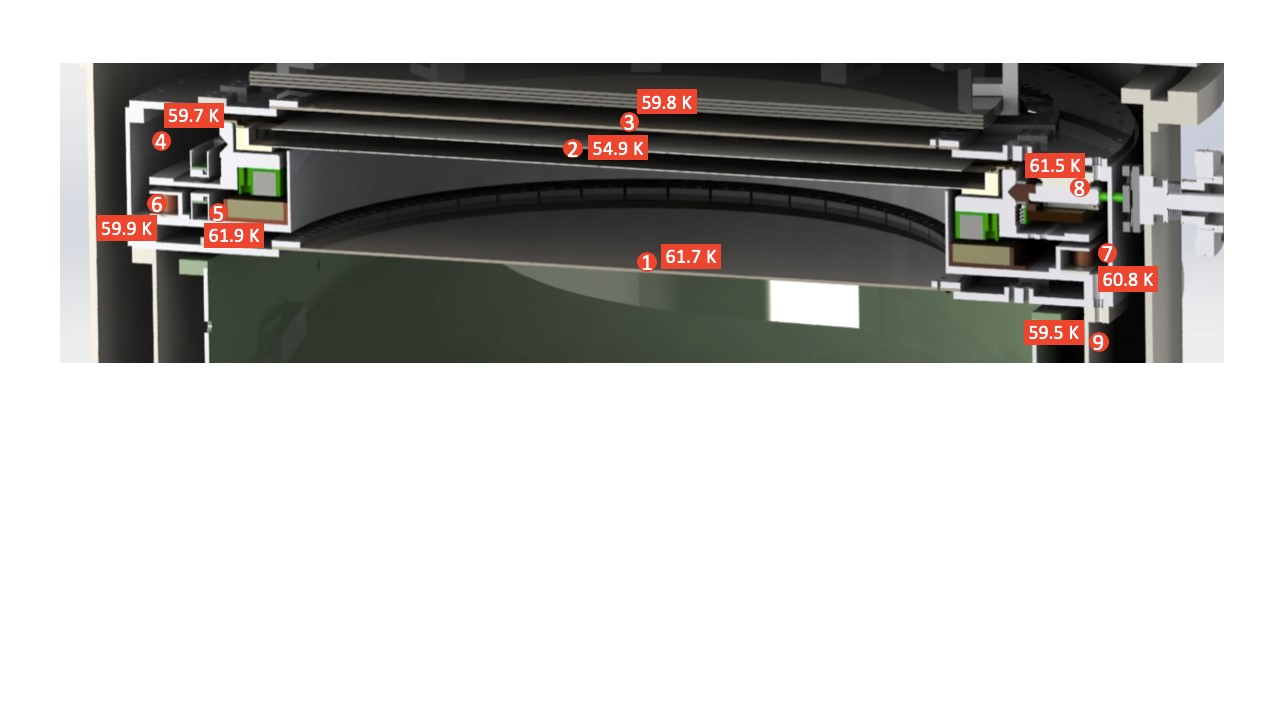
\includegraphics[width=0.98\linewidth, trim=2cm 9cm 2cm 0cm, clip]{CHWPEvaluation/Figures/chwp_temperatures.jpg}
    \caption[CHWP temperatures]{The temperatures of the various CHWP components after integration with the optics tube. The alumina filter temperature is close to that of the PTC shell, and the stator is well thermalized. The rotor temperature is close to that of the alumina filter, while cooling slightly lower due to radiative coupling to the 4 K field lens.}
    \label{fig:chwp_temperatures}
\end{figure}

Third, we search for any CHWP-induced heating of the focal plane. We spin the rotor up and down at various drive voltages over several hours in the UCSD setup, and we see no changes in mK temperatures to within a $\approx$~0.3~mK/hr background drift,\footnote{No focal plane temperature regulation was employed during this test, and therefore this background drift is larger than that which is achievable.} implying negligible CHWP-induced focal-plane vibrations. This null result is expected, as the CHWP's resonant frequency $\sqrt{k / m} \approx$~130~Hz is much higher than its $\approx$~2~Hz rotation frequency.

%%%%%%%%%%%%%%%%%%%%%%%%%%%%%%%%
%%%%%%%%%%%%%%%%%%%%%%%%%%%%%%%%

\subsection{Shutdown and recovery}
\label{sec:pb2a_chwp_evaluation_shutdown_recovery}

A critical capability for long-term field operation is the clean recovery of the rotor following a power disruption. When the optics tube's PTR shuts off, the CHWP warms with the rest of the experiment, and in the absence of a robust recovery procedure, the rotor may become difficult to recenter without opening the cryostat. Therefore, we employ two redundant procedures to recapture the CHWP in the event of a cryostat warmup.

The primary procedure is to stop and grip the rotor before the 50~K stage warms appreciably. The CHWP electronics are powered via an uninterrupted power supply (UPS) that provides a $\sim$~30~min window after site-wide power loss during which the CHWP must be stilled, re-gripped, and stowed. Necessitated by its low friction, the rotor is actively braked by globally inverting the motor's H-driver outputs (see Section~\ref{sec:driver}). Figure~\ref{fig:spin_down} shows rotation frequency vs. time for various braking voltages, and the measured spin-down time is $\approx$~5~min, which is sufficiently shorter than the UPS duration. After rotation stops, the rotor is gripped loosely to provide a margin for thermal expansion, the gripper motors' brakes are applied, and the CHWP electronics are shut down. When site power is later restored, the cooldown procedure in Section~\ref{sec:pb2a_chwp_evaluation_start_up} commences, and nominal CHWP operation resumes. We have tested this emergency stop and re-grip procedure multiple times in the LBNL cryostat and have shown that it keeps the rotor centered to within 0.5~mm.

In the event of an issue when stopping and re-gripping, we employ a backup procedure to recover the rotor after it has ``fallen.'' As shown in Figure~\ref{fig:chwp_tabletop}, the retaining ring includes six PTFE crash pads designed to gently ``catch'' the rotor and limit its misalignment after the bearing disengages. Once site power is restored, we orient the receiver horizontally, as shown in Figure~\ref{fig:chwp_in_pb2b}, lift the rotor along the $+y$ direction using the bottom gripper finger (see Section~\ref{sec:gripper_design}), and then grab it using the top two fingers. This after-the-fact technique is less than ideal, as it requires the rotor to be secured and realigned from an indeterminate position. Nonetheless, it provides necessary insurance against opening the cryostat, which is an expensive operation. We have tested this backup procedure in the LBNL and UCSD cryostats and have shown it to recenter the rotor to within 1.5~mm of its original position, which is good enough to reattain 2~Hz rotation.

\begin{figure}[!t]
    \centering
    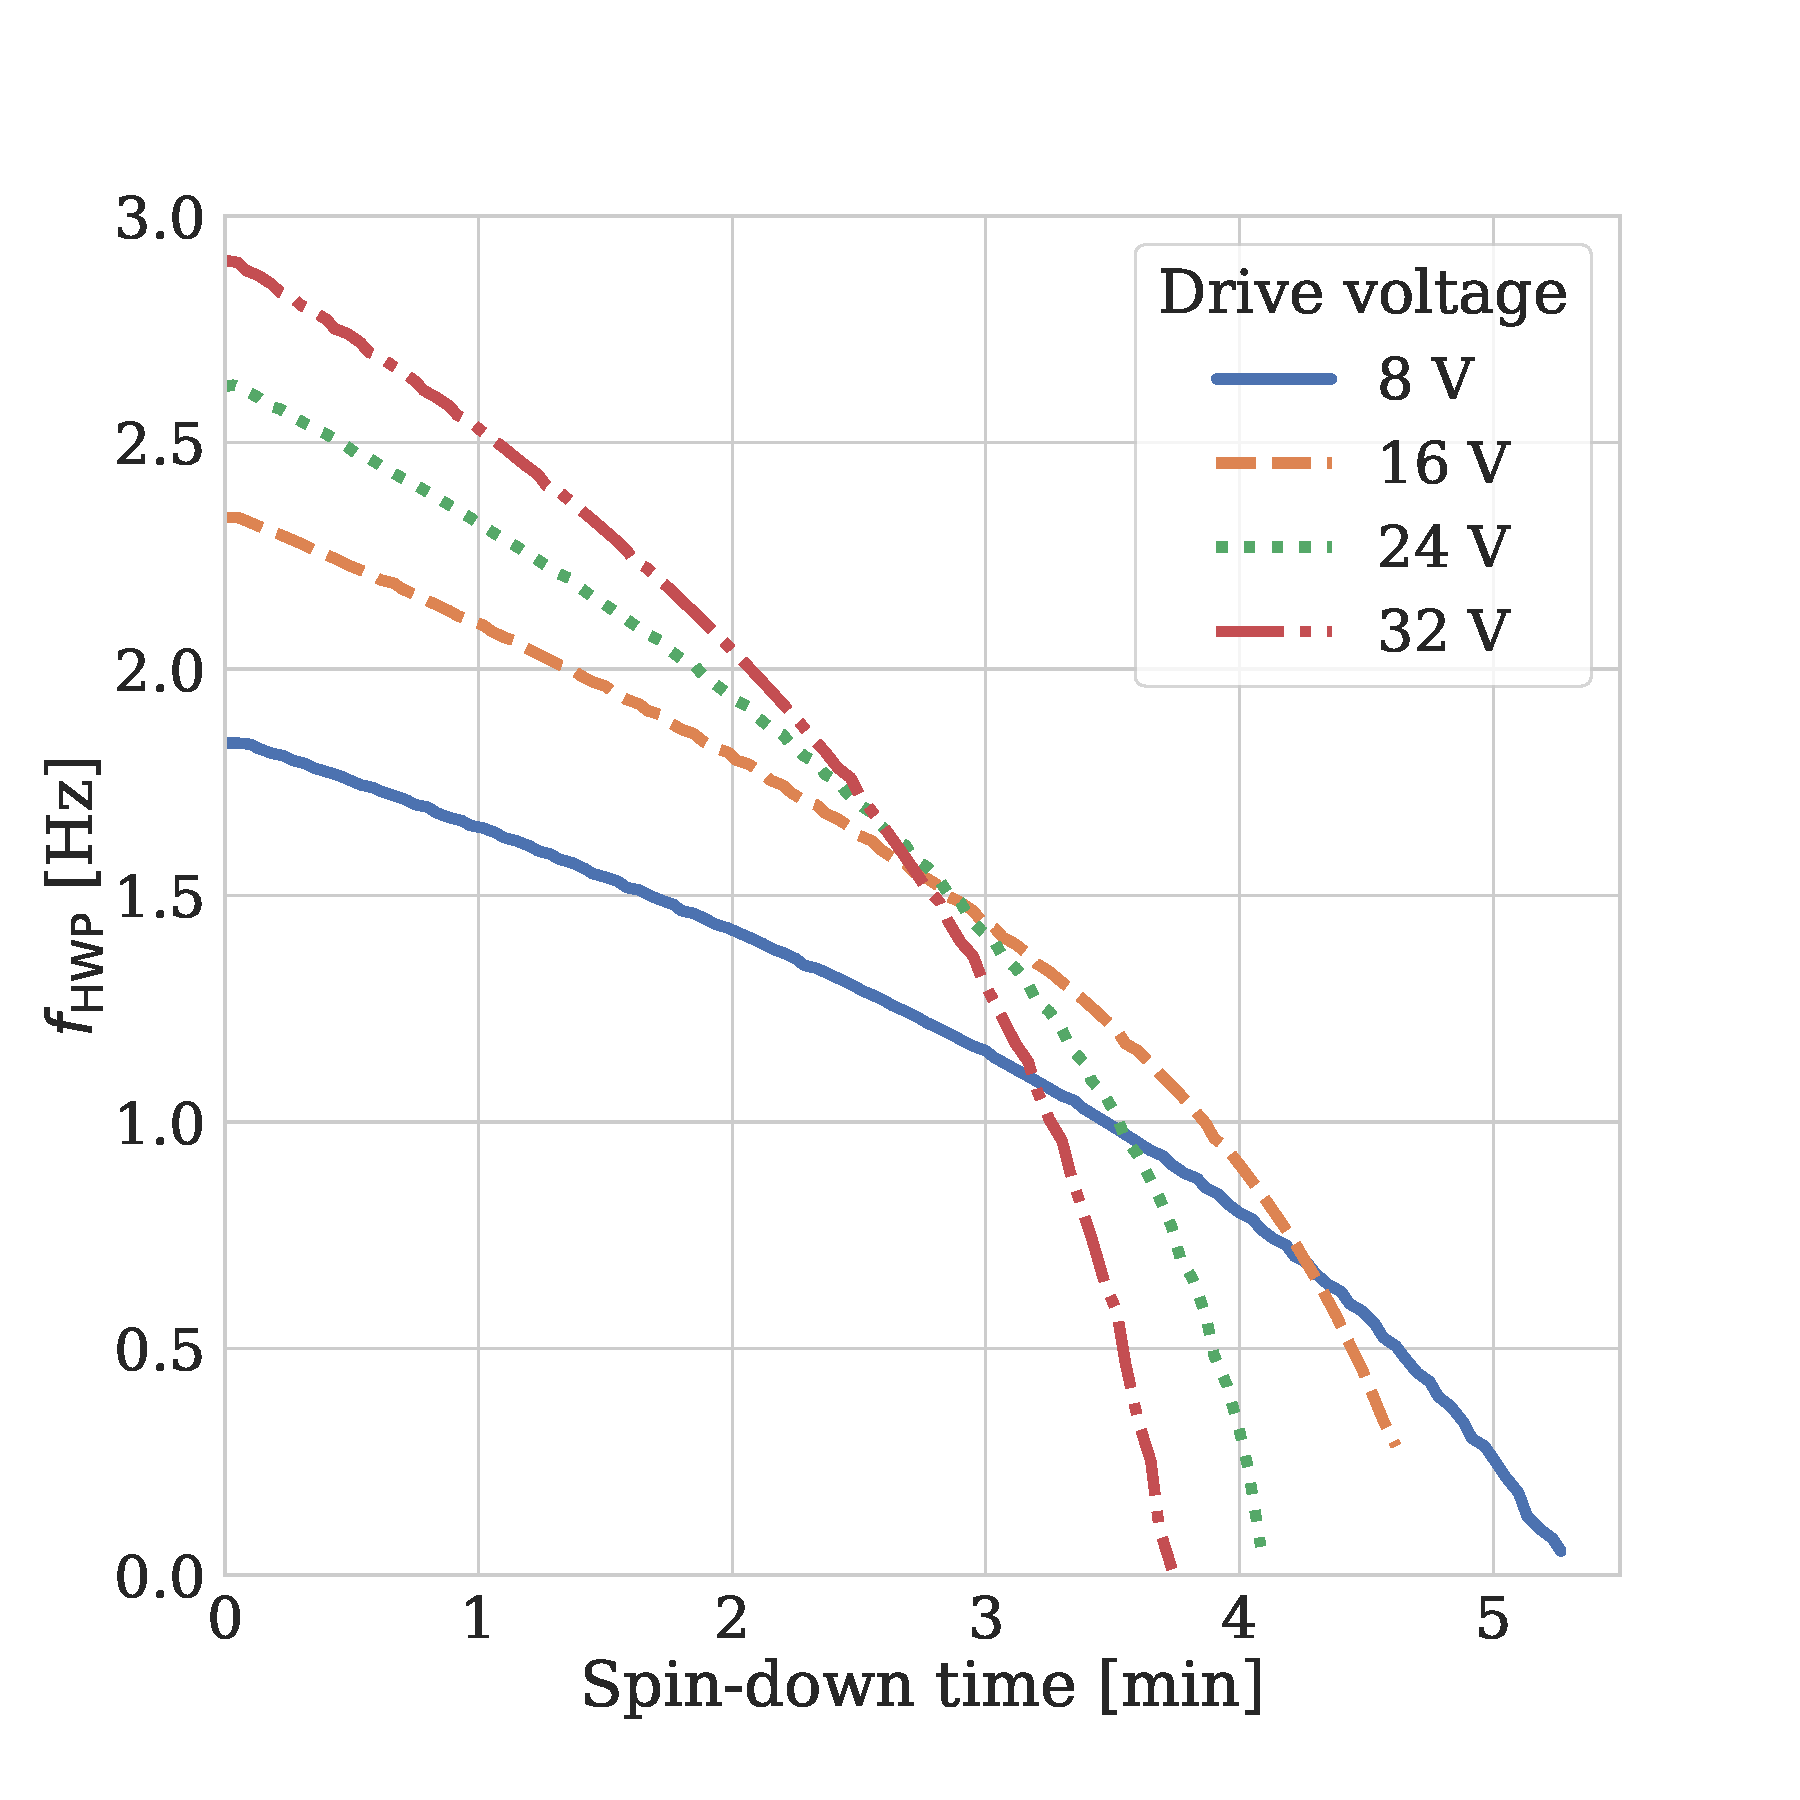
\includegraphics[width=0.6\linewidth, trim=0.3cm 0.9cm 3.0cm 3.3cm, clip]{CHWPEvaluation/Figures/rotor_spindown_brake.pdf}
    \caption{Spin-down tests from various rotation frequencies using various braking voltages. These tests did not employ the PID controller, which will shorten the stopping time for continuous rotation frequencies $<$~2.8~Hz.}
    \label{fig:spin_down}
\end{figure}

%%%%%%%%%%%%%%%%%%%%%%%%%%%%%%%%
%%%%%%%%%%%%%%%%%%%%%%%%%%%%%%%%
%%%%%%%%%%%%%%%%%%%%%%%%%%%%%%%%

\section{Data quality}
\label{sec:pb2b_chwp_data_quality}

In this section, we review the impact of the CHWP on experiment data quality within the context of the noise requirements presented in Section~\ref{sec:noise_requirements}. Specifically, we discuss encoder jitter, magnetic interference, and rotor temperature stability, highlighting the achieved values in Table~\ref{tab:requirements}.

%%%%%%%%%%%%%%%%%%%%%%%%%%%%%%%%
%%%%%%%%%%%%%%%%%%%%%%%%%%%%%%%%

\subsection{Angle encoder performance}
\label{sec:pb2b_chwp_evaluation_encoder_jitter}

We use the same hour-long data set presented in Section~\ref{sec:continuous_rotation} to evaluate the angle encoder described in Section~\ref{sec:angle_encoder}. For purely historical reasons, this test is performed using an Arduino MCU,\footnote{Arduino Leonardo: https://store.arduino.cc/usa/arduino-leonardo-eth} which employs two separate 16~MHz clocks, instead of the BBB, which employs one shared 200~MHz clock. Additionally, this test did not utilize PID control and therefore relies on open-loop motor stability to maintain steady rotation. Our primary goal in this section is to measure the angle encoder's white noise level and compare it to the $\ll$~$3$~$\mathrm{\mu rad / \sqrt{Hz}}$ requirement in Table~\ref{tab:requirements}.

As described in Section~\ref{sec:angle_encoder}, the rotor angle $\chi(t)$ is reconstructed by linearly interpolating angle encoder ticks to IRIG time $t$ as
\begin{equation}
    \chi(\tau_{\mathrm{Enc}}) \longleftrightarrow t(\tau_{\mathrm{IRIG}}) \, ,
    \label{eq:interpolation}
\end{equation}
where $\tau_{\mathrm{Enc}}$ and $\tau_{\mathrm{IRIG}}$ are the MCU clocks for the encoder and IRIG signals, respectively. Deviations between $\tau_{\mathrm{Enc}}$ and $\tau_{\mathrm{IRIG}}$ on the Arduino lead to additional noise that will not exist when using the BBB in the field. Therefore, we analyze both $\chi(t)$ and $\tau_{\mathrm{IRIG}}(t)$ to distinguish MCU drifts from those of the rotation mechanism and encoder system.

To facilitate the following discussion, we consider two illustrative angle jitter definitions: the residual after subtracting a quadratic fit
\begin{equation}
\delta \chi_{\mathrm{HWP}}^{\mathrm{poly}}(t) = \chi(t) - P_{\mathrm{2}}^{\mathrm{\chi}}(t) \, ,
\label{eq:angle_poly_jitter}
\end{equation}
\noindent
and the residual after subtracting a quadratic fit plus an angle-dependent function $A(\chi)$
\begin{equation}
    \delta \chi_{\mathrm{HWP}}^{\mathrm{temp}}(t) = \chi(t) - \left[ P_{2}^{\chi}(t) + A(\chi) \right] \, .
\label{eq:angle_temp_jitter}
\end{equation}
\noindent
For this test data, we select a simple $2 \pi$-repeating template
\begin{equation}
    A(\chi) = A(\chi - 2 \pi n) \; ; \; n \in \{0, 1, \cdots, N_{\mathrm{rev}} \} \, ,
    \label{eq:template}
\end{equation}
where $N_{\mathrm{rev}}$ is the number of completed revolutions in the data set and where $A(\chi - 2 \pi n)$ is constructed by taking a window-weighted average of the encoder pattern over all $N_{\mathrm{rev}}$. In practice, a more complex function can be used to remove HWP-synchronous signals in the field \cite{essinger-hileman_systematic_2016}, but a uniform template works well for lab characterization. Additionally, we define IRIG clock jitter as
\begin{equation}
    \delta \tau_{\mathrm{IRIG}}^{\mathrm{poly}}(t) = \tau_{\mathrm{IRIG}}(t) - P_{2}^{\tau}(t) \, ,
\end{equation}
which we use to evaluate MCU clock drifts.

A three-second segment of angle jitters $\delta \chi_{\mathrm{HWP}}^{\mathrm{poly}}$ and $\delta \chi_{\mathrm{HWP}}^{\mathrm{temp}}$ are shown in the top panel of Figure~\ref{fig:jitter_psd}. The polynomial-subtracted spectrum $\delta \chi_{\mathrm{HWP}}^{\mathrm{poly}}$ shows a distinct peak-to-peak variation of $\approx$~1~mrad at $f_{\mathrm{HWP}}$ in addition to higher-order structures, and the template-subtracted spectrum $\delta \chi_{\mathrm{HWP}}^{\mathrm{temp}}$ shows that most of this jitter is removed by $A(\chi)$. A unique property of the SMB is that it does not wobble, even if it is gravitationally imbalanced. Therefore the observed $\delta \chi_{\mathrm{HWP}}^{\mathrm{poly}}$ signal is caused by a slight misalignment between the slotted encoder plate and magnet ring, while higher-frequency structures are caused by non-uniform patterning of the encoder slots. Three seconds of IRIG clock jitter $\delta \tau_{\mathrm{IRIG}}^{\mathrm{poly}}$ is also shown in Figure~\ref{fig:jitter_psd} and is effectively a measurement of Arduino clock noise. Because the IRIG signal is GPS synchronized to $\leq$~40~ns, the observed drift is due to instability of the Arduino's crystal oscillators, which we discuss further below.

Power spectral densities (PSDs) of the angle and clock jitters are shown in the bottom panel of Figure~\ref{fig:jitter_psd}. The sharpness of the peaks in the $\delta \chi_{\mathrm{HWP}}^{\mathrm{poly}}$ spectrum demonstrates excellent rotational stability, and the suppression of those peaks in the $\delta \chi_{\mathrm{HWP}}^{\mathrm{temp}}$ spectrum confirms that $A(\chi)$ measures all but a few $\delta \chi_{\mathrm{HWP}}$ features with high signal-to-noise. The $A(\chi)$ subtraction also suppresses side-band power in the $f_{\mathrm{HWP}}$ harmonics, better revealing a white-noise level of $\approx \: 0.1 \; \mathrm{\mu rad / \sqrt{Hz}}$.

Both $\delta \chi_{\mathrm{HWP}}$ spectra have a 1/f knee of $\approx$~1~Hz, which is larger than expected from the $\Delta f_{\mathrm{HWP}}$ measurement in Figure~\ref{fig:rot_stability}. Therefore, we compare the angle and IRIG spectra to analyze the contribution of MCU clock drifts to the observed 1/f noise. The two MCU clocks, $\tau_{\mathrm{IRIG}}$ and $\tau_{\mathrm{Enc}}$ (see Equation~\ref{eq:interpolation}), fluctuate with $\approx$~90\% coherence, and because common-mode clock drifts are subtracted during angle-time interpolation, $\delta \chi_{\mathrm{HWP}}$ 1/f power dips beneath that of $2 \pi f_{\mathrm{HWP}} \delta \tau_{\mathrm{IRIG}}^{\mathrm{poly}}$ between $\approx$~0.05~Hz and the IRIG's 0.5~Hz Nyquist frequency. Below $\approx$~0.05~Hz, drifts in rotational velocity begin to contribute and the $\delta \chi_{\mathrm{HWP}}$ spectra steepen, but even so, MCU-induced 1/f noise remains dominant down to $\sim$~0.01~Hz. This finding  motivated us to replace the Arduino with the BBB, which uses a single shared clock ($\tau_{\mathrm{Enc}} = \tau_{\mathrm{IRIG}}$) and has a measured 1/f knee of <~0.1~Hz. This configuration allows the 1~Hz IRIG signal to fully subtract MCU clock drifts during angle-time interpolation, and therefore we expect significantly improved low-frequency noise when measuring $\chi(t)$ in the field.

\begin{figure}[!t]
    \centering
    \subfloat[\label{fig:jitter_psd:a}]{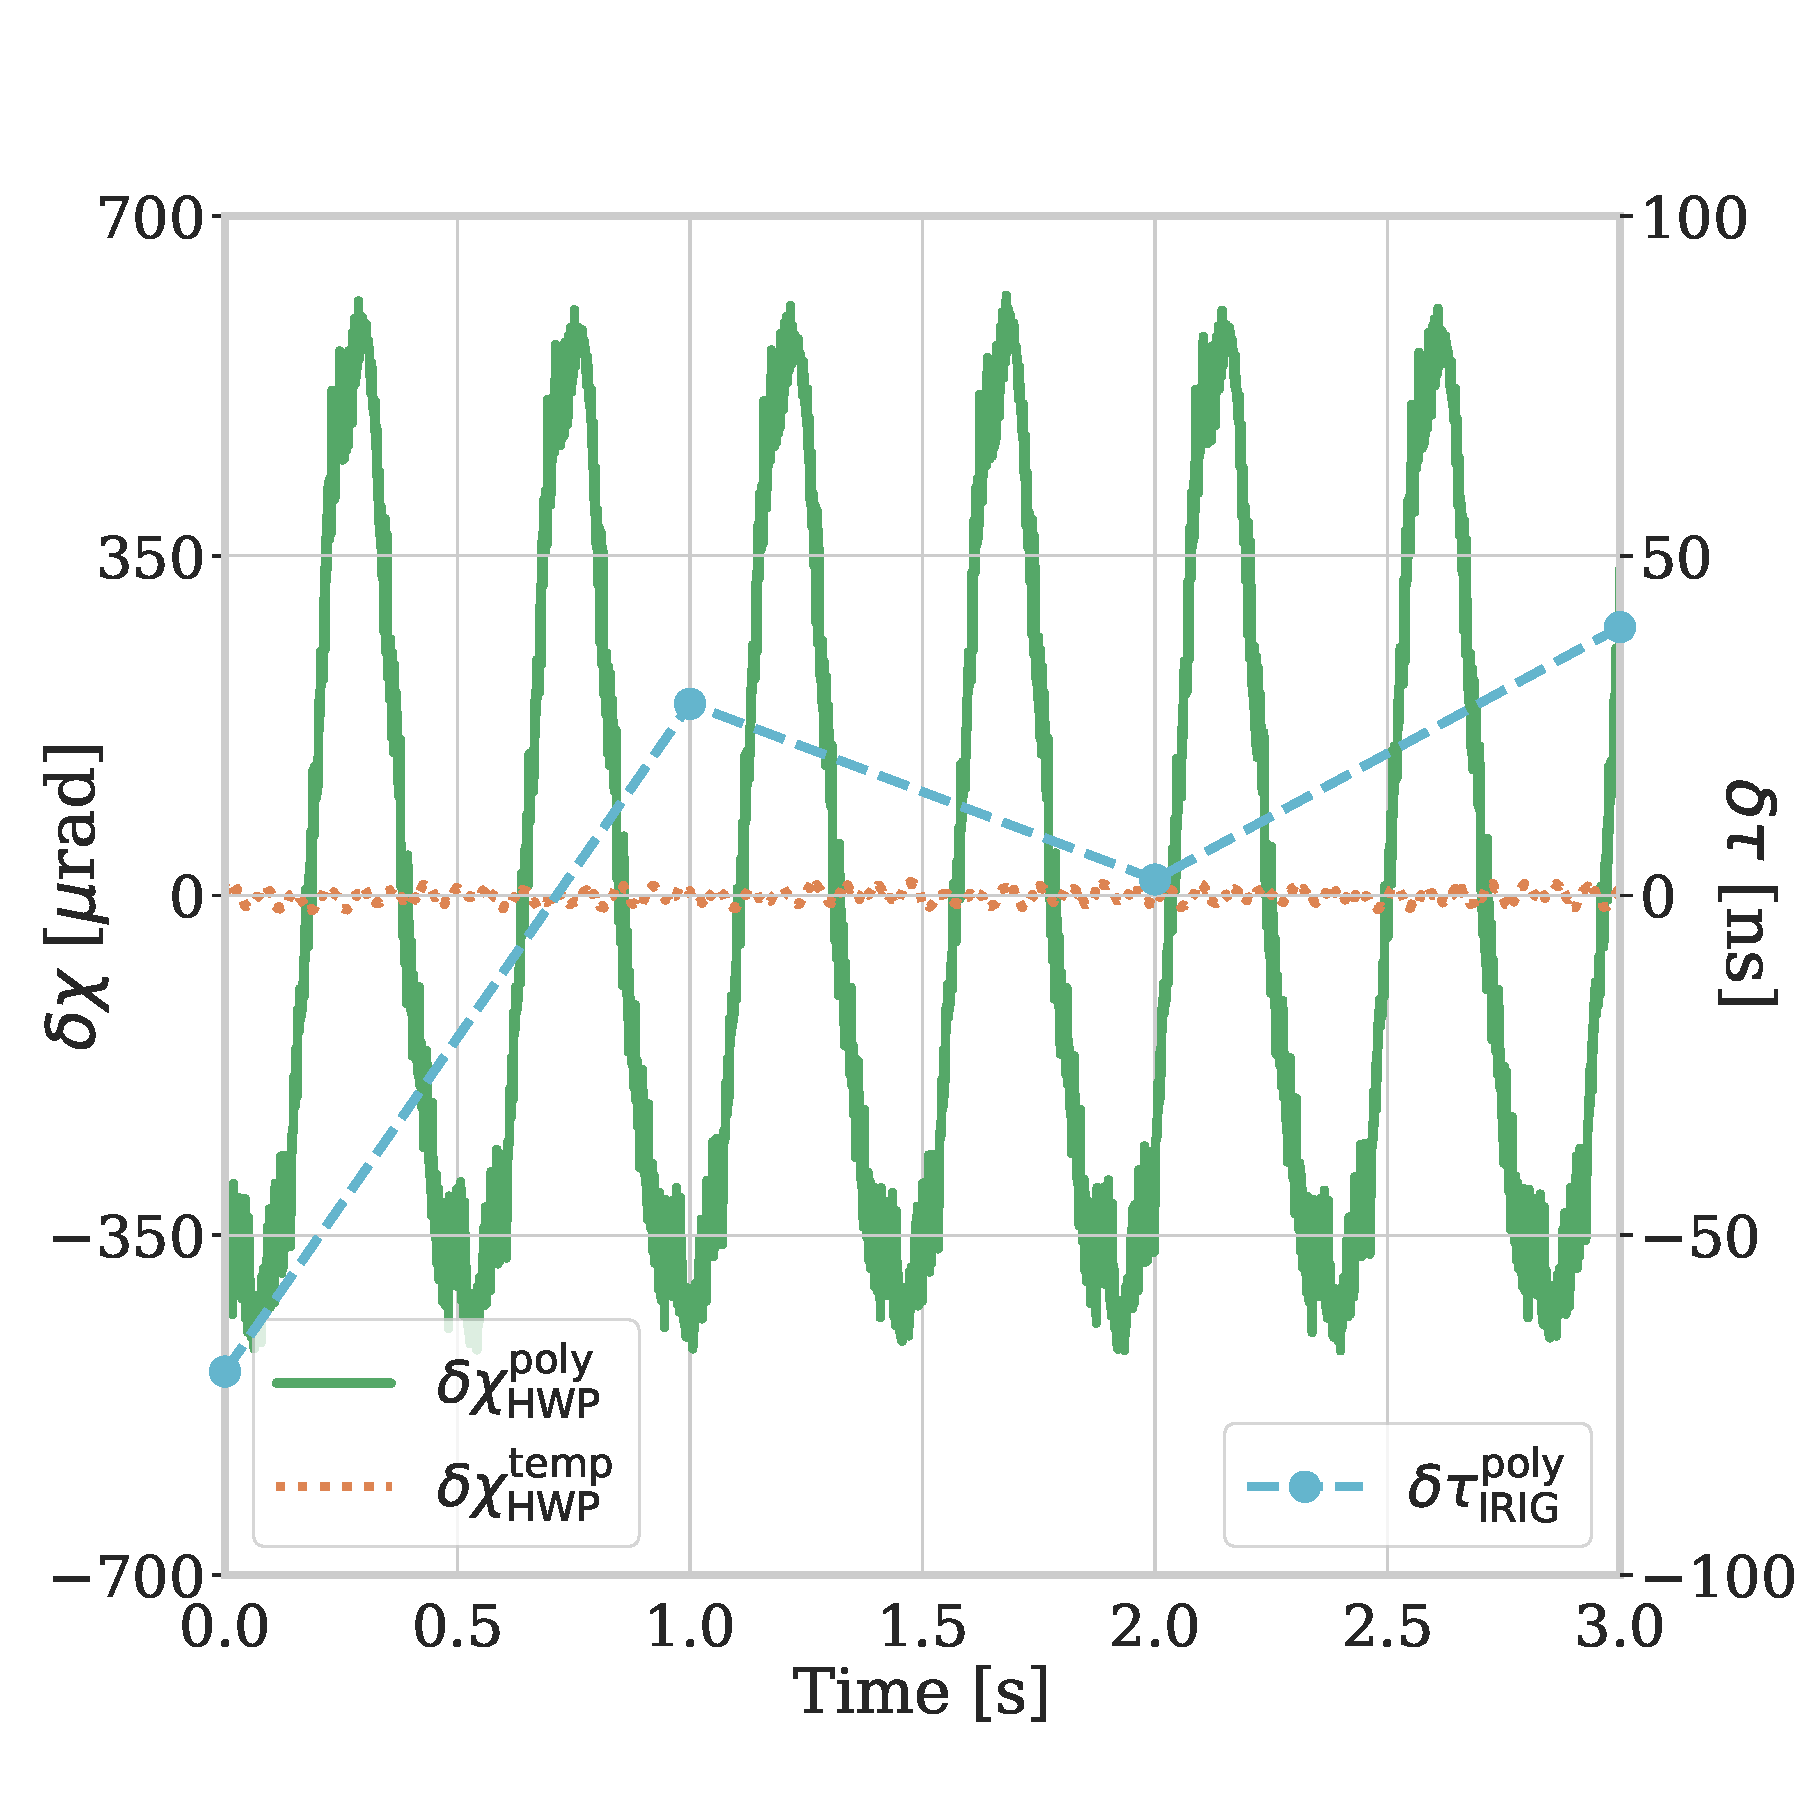
\includegraphics[width=0.49\linewidth, trim=0.8cm 1cm -0.4cm 3cm, clip]{CHWPEvaluation/Figures/encoderJitter_tod.pdf}}
    \subfloat[\label{fig:jitter_psd:b}]{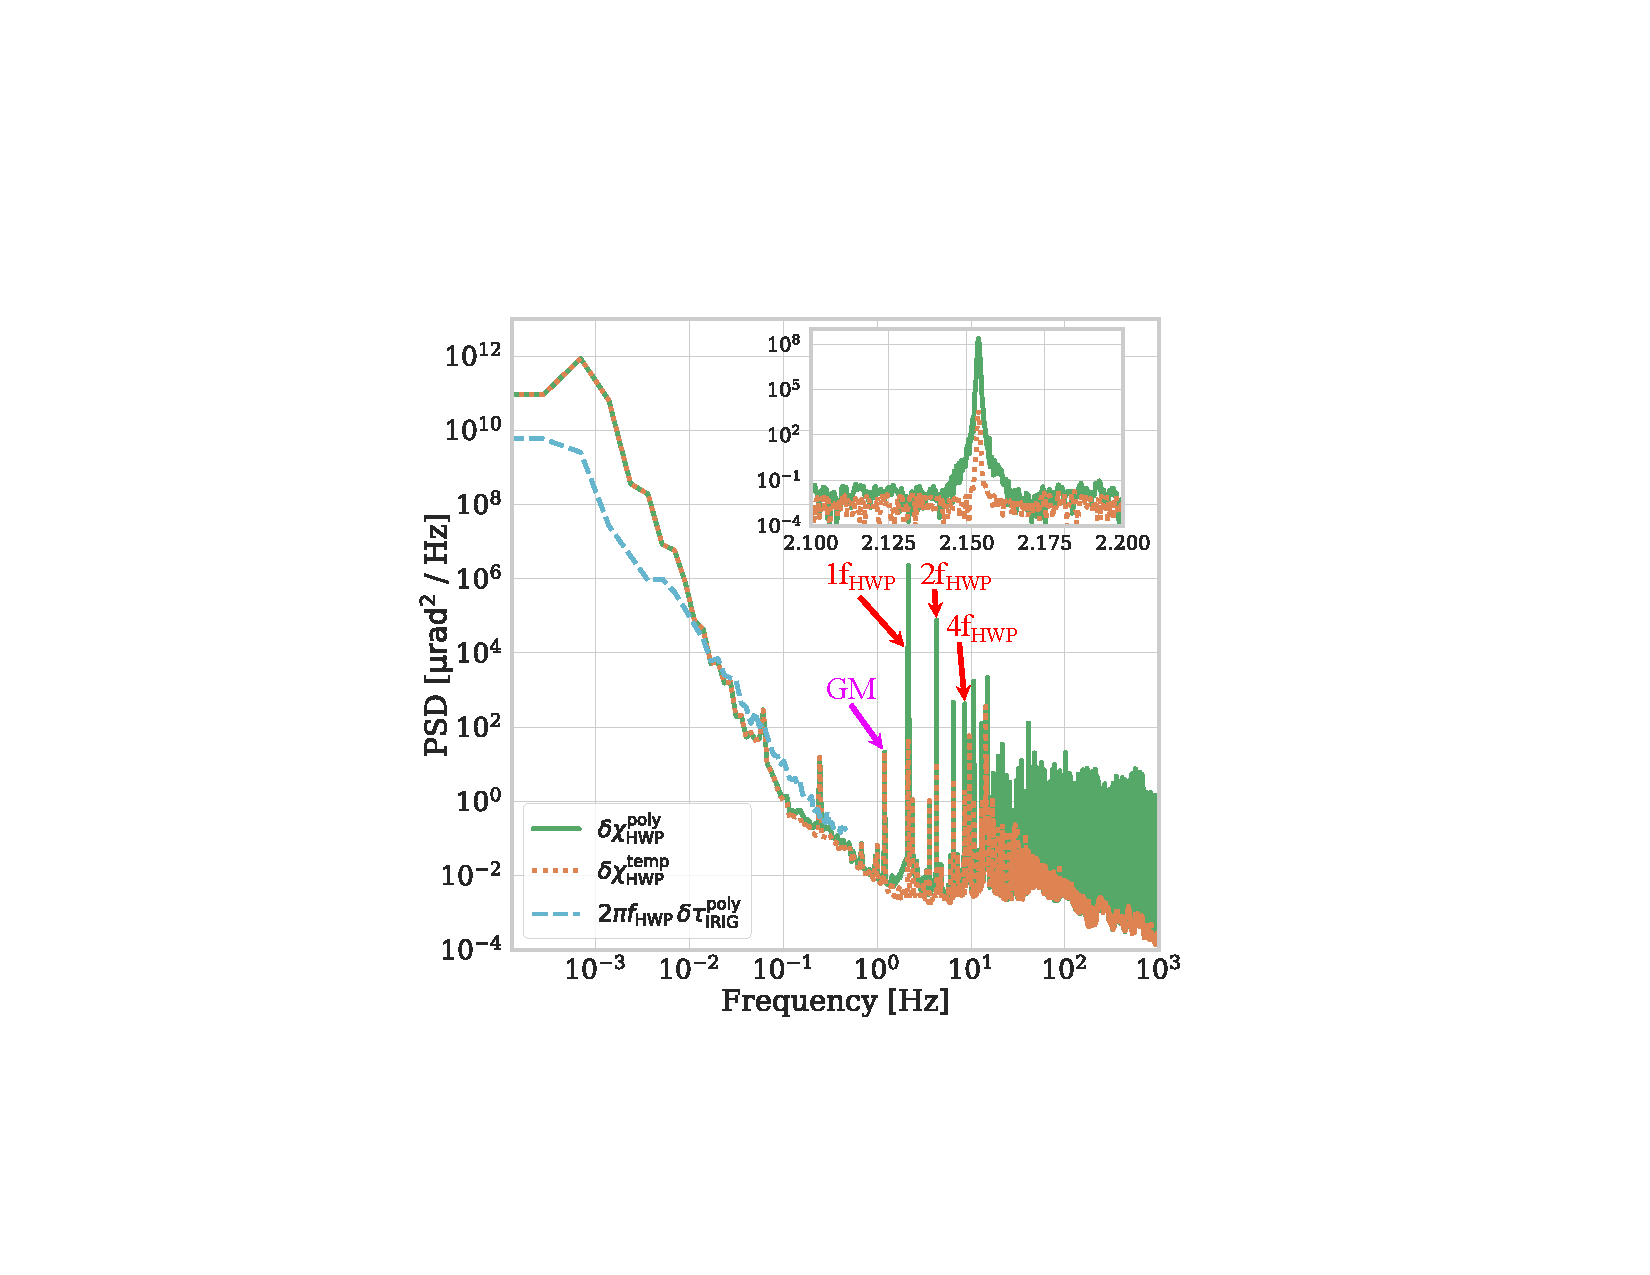
\includegraphics[width=0.47\linewidth, trim=7cm 4.3cm 7.9cm 5.2cm, clip]{CHWPEvaluation/Figures/encoderJitter_psd.pdf}}
    \caption{A measurement of encoder performance during 1 hour of testing in the LBNL setup. \textbf{Top panel:} a three-second sample of the angle and IRIG jitters. The rotor is spinning at $\approx$~2.15~Hz and its angle is sampled 1,140 times per revolution. \textbf{Bottom panel:} PSDs of the angle and IRIG jitters, including a zoomed inset of the $1 f_{\mathrm{HWP}}$ peak with finer binning. We multiply $\delta \tau_{\mathrm{IRIG}}^{\mathrm{poly}}$ by $2 \pi f_{\mathrm{HWP}}$ to covert it from seconds to radians.}
    \label{fig:jitter_psd}
\end{figure}

%%%%%%%%%%%%%%%%%%%%%%%%%%%%%%%%
%%%%%%%%%%%%%%%%%%%%%%%%%%%%%%%%

\subsection{Magnetic interference}
\label{sec:pb2b_chwp_evaluation_magnetic_interference}

The CHWP's motor and rotor both introduce magnetic interference that can affect the detectors and their SQUID amplifiers. In particular, interference at 4$f_{\mathrm{HWP}}$ mimics a sky signal and must be especially well controlled. The motor energizes three phases across 114 solenoids at 38$f_{\mathrm{HWP}}$, and its large multipole number causes its $\approx$ 20~G field to decay quickly with distance. The magnet ring, on the other hand, has only 16 segments---resulting in a lower multipole number---and a surface magnetization of $\approx$~5,000~G, posing a greater 4$f_{\mathrm{HWP}}$ interference concern. 

Magnetic field testing is performed at LBNL using a room-temperature magnetometer\footnote{Honeywell HMR2300: https://aerospace.honeywell.com/} placed 1.5~m behind the CHWP assembly at the approximate location of a detector near the edge of the focal plane\footnote{We calculate that CHWP-induced magnetic fields are larger near the edge of the focal plane than near the center. Therefore, this measurement represents a worst-case scenario for potential detector interference.} (see Figure~\ref{fig:pb2_telescope}). The CHWP rotates steadily at $\approx$~2.15~Hz, and the ambient magnetic field is measured at 150 samples per second for 100~s. The results are presented in Figure~\ref{fig:mag_spec}. The time-ordered data show a DC field of 926~mG\footnote{This average field applies a $\approx$~-0.3~mK DC shift to the TES transition temperature $T_{\mathrm{c}}$, which is less than $T_{\mathrm{c}}$ variation across the focal plane \cite{westbrook_polarbear-2_2018} and is calibrated out during detector tuning.} and a $\approx 5$~mG oscillation at $1 f_{\mathrm{HWP}}$, while the spectrum shows peaks at $1 f_{\mathrm{HWP}}$, $2 f_{\mathrm{HWP}}$, and at harmonics of the GM cooler's cycle frequency. However, the $4 f_{\mathrm{HWP}}$ component lies beneath the noise floor, setting a bound on its amplitude of $< \: 10 \; \mathrm{\mu G / \sqrt{Hz}}$.

\begin{figure}[!t]
    \centering
    \subfloat[\label{fig:mag_spec:a}]{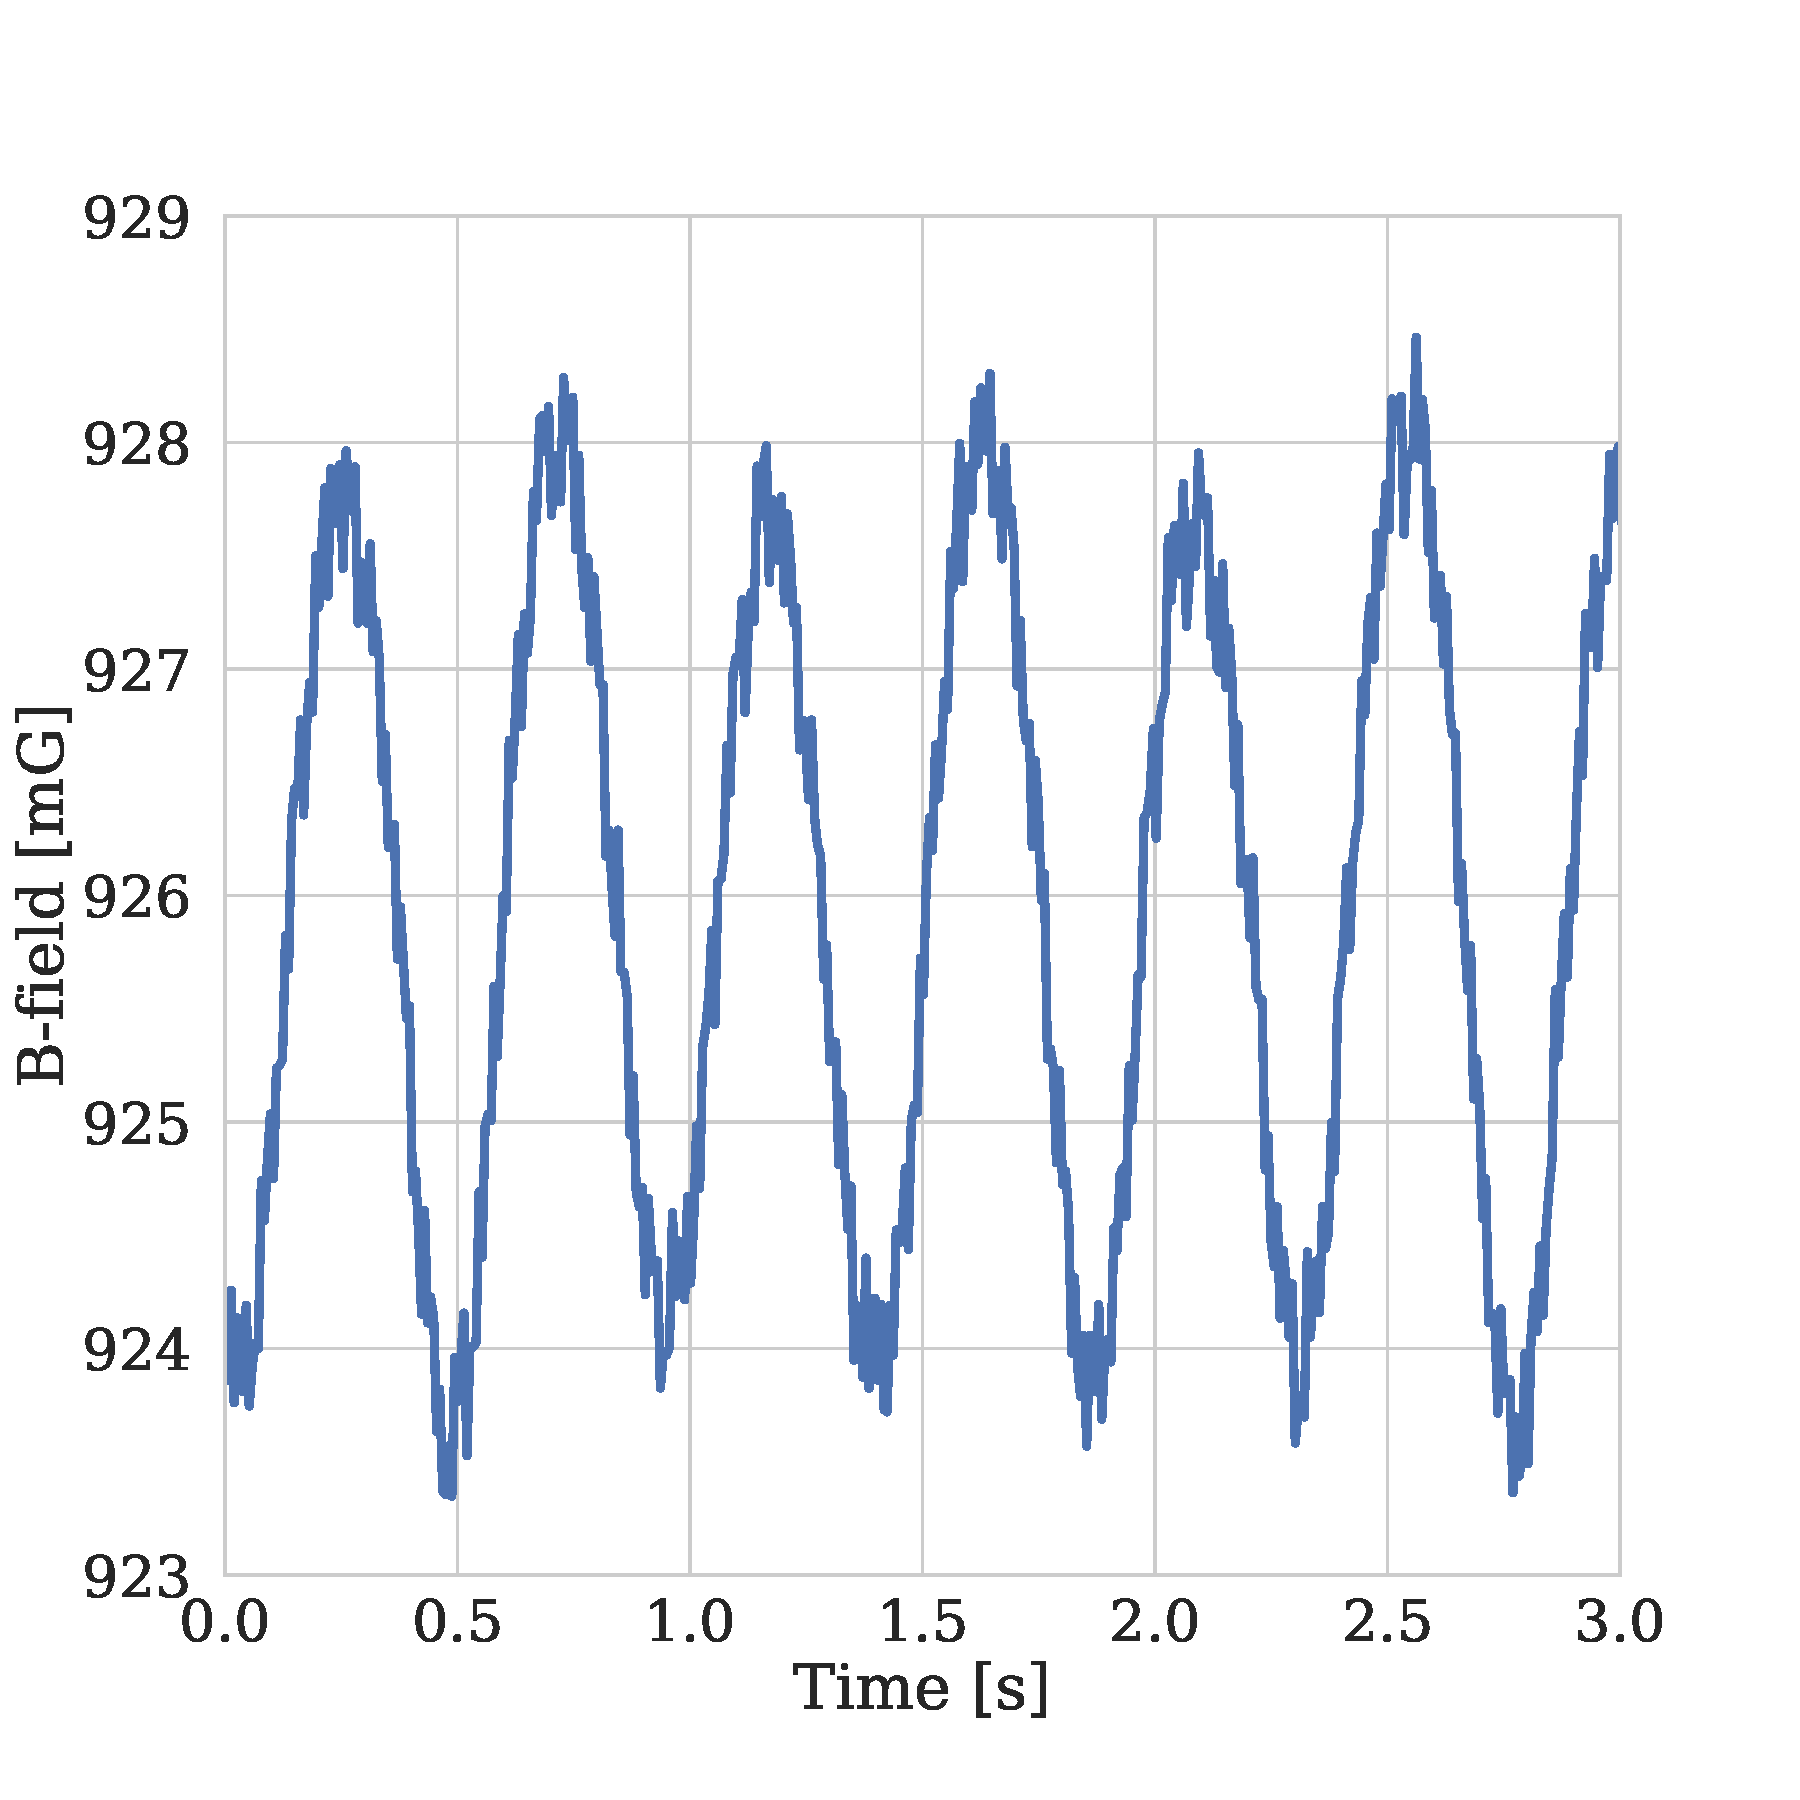
\includegraphics[width=0.46\linewidth, trim=0cm 1cm 2cm 2.5cm, clip]{CHWPEvaluation/Figures/bfieldJitter_tod.pdf}}
    \subfloat[\label{fig:mg_spec:b}]{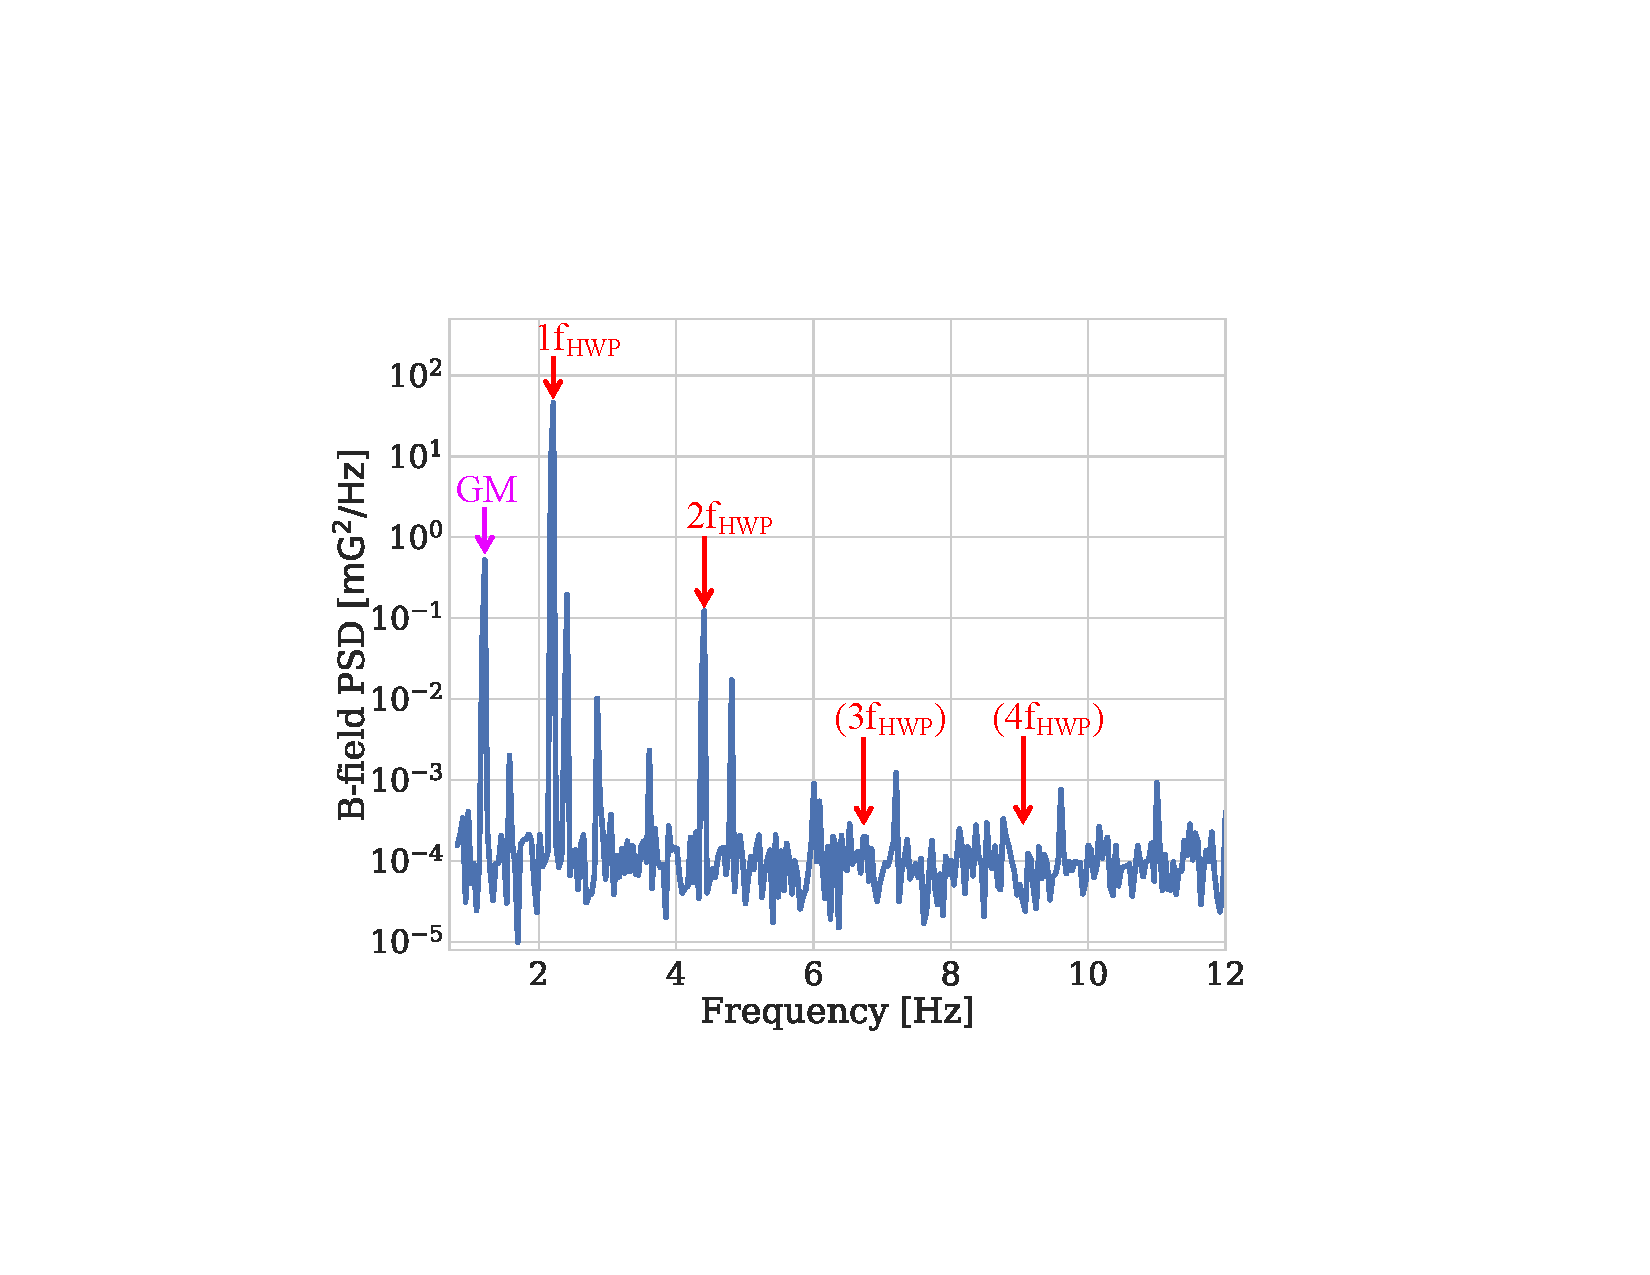
\includegraphics[width=0.50\linewidth, trim=5.5cm 3.8cm 6.9cm 5cm, clip]{CHWPEvaluation/Figures/bfieldJitter_psd.pdf}}
    \caption{A measurement of the magnetic field 1.5~m behind the CHWP assembly during 100~s of continuous rotation at 2.15~Hz in the LBNL cryostat. \textbf{Top panel:} 3~s of time-ordered magnetometer data, showing a clear $\approx$~5~mG peak-to-peak variation at 1$f_{\mathrm{HWP}}$. \textbf{Bottom panel:} the B-field's power spectral density. Red arrows mark rotation-synchronous peaks, while the magenta arrow marks that of the GM cooler. The unmarked peaks are environmental and are predominantly GM harmonics.}
    \label{fig:mag_spec}
\end{figure}

Full-system interference testing is performed at UCSD by monitoring detector outputs when the CHWP is spinning. During two minutes of rotation at 2~Hz, data is collected from both optical and non-optical bolometers across the full focal plane. While $2 f_{\mathrm{HWP}}$ and $4 f_{\mathrm{HWP}}$ signals are visible in the optical detectors, as expected, no CHWP-induced signals are detected in any of the dark detectors. In addition, because 4$f_{\mathrm{HWP}}$ magnetic interference is $\leq \; 10^{-6}$ that at 1$f_{\mathrm{HWP}}$, as shown in Figure~\ref{fig:mag_spec}, this test also suggests that no 4$f_{\mathrm{HWP}}$ magnetic features will arise when $\sim \: 5 \times 10^{3}$ detectors are coadded during data analysis.

%%%%%%%%%%%%%%%%%%%%%%%%%%%%%%%%
%%%%%%%%%%%%%%%%%%%%%%%%%%%%%%%%

\subsection{Rotor temperature stability}
\label{sec:pb2b_chwp_evaluation_rotor_temperature_stability}

To evaluate thermal stability, we simulate rotor temperature using the thermal model presented in Section~\ref{sec:thermal_design}. Because it is floating, the rotor's temperature variations are dominated by those of the 50~K stage to which it is radiatively tied. These CHWP fluctuations are expected to be very slow, as the rotor has a $\approx$~900~J/K heat capacity at base temperature and a $\approx$~10~mW/K coupling to its 50~K surroundings. Due to diurnal variations in ambient temperature and changes in telescope elevation---which impact PTR performance---50~K temperature drifts in Chile are substantially larger than those in the lab. Therefore, we use 24 hours of 50~K temperature data from PB-2a, which is operating in the field, to simulate the expected rotor stability. The selected PB-2a data includes telescope slew testing, and therefore the presented 50~K-stage variations represent an upper bound on those expected during science observations.

The measured 50~K-stage and simulated rotor PSDs are shown in Figure~\ref{fig:hwp_stability}. The rotor acts as a low-pass filter, and its simulated drift is $\approx$~0.3~$\mathrm{mK / \sqrt{Hz}}$ at 1~mHz, which is below the 1~$\mathrm{mK / \sqrt{Hz}}$ requirement in Tab.~\ref{tab:requirements}. We note that rotor temperature stability can be substantially improved by regulating the 50~K-stage temperature, which may become necessary for future experiments with tighter noise requirements.

\begin{figure}[!t]
    \centering
    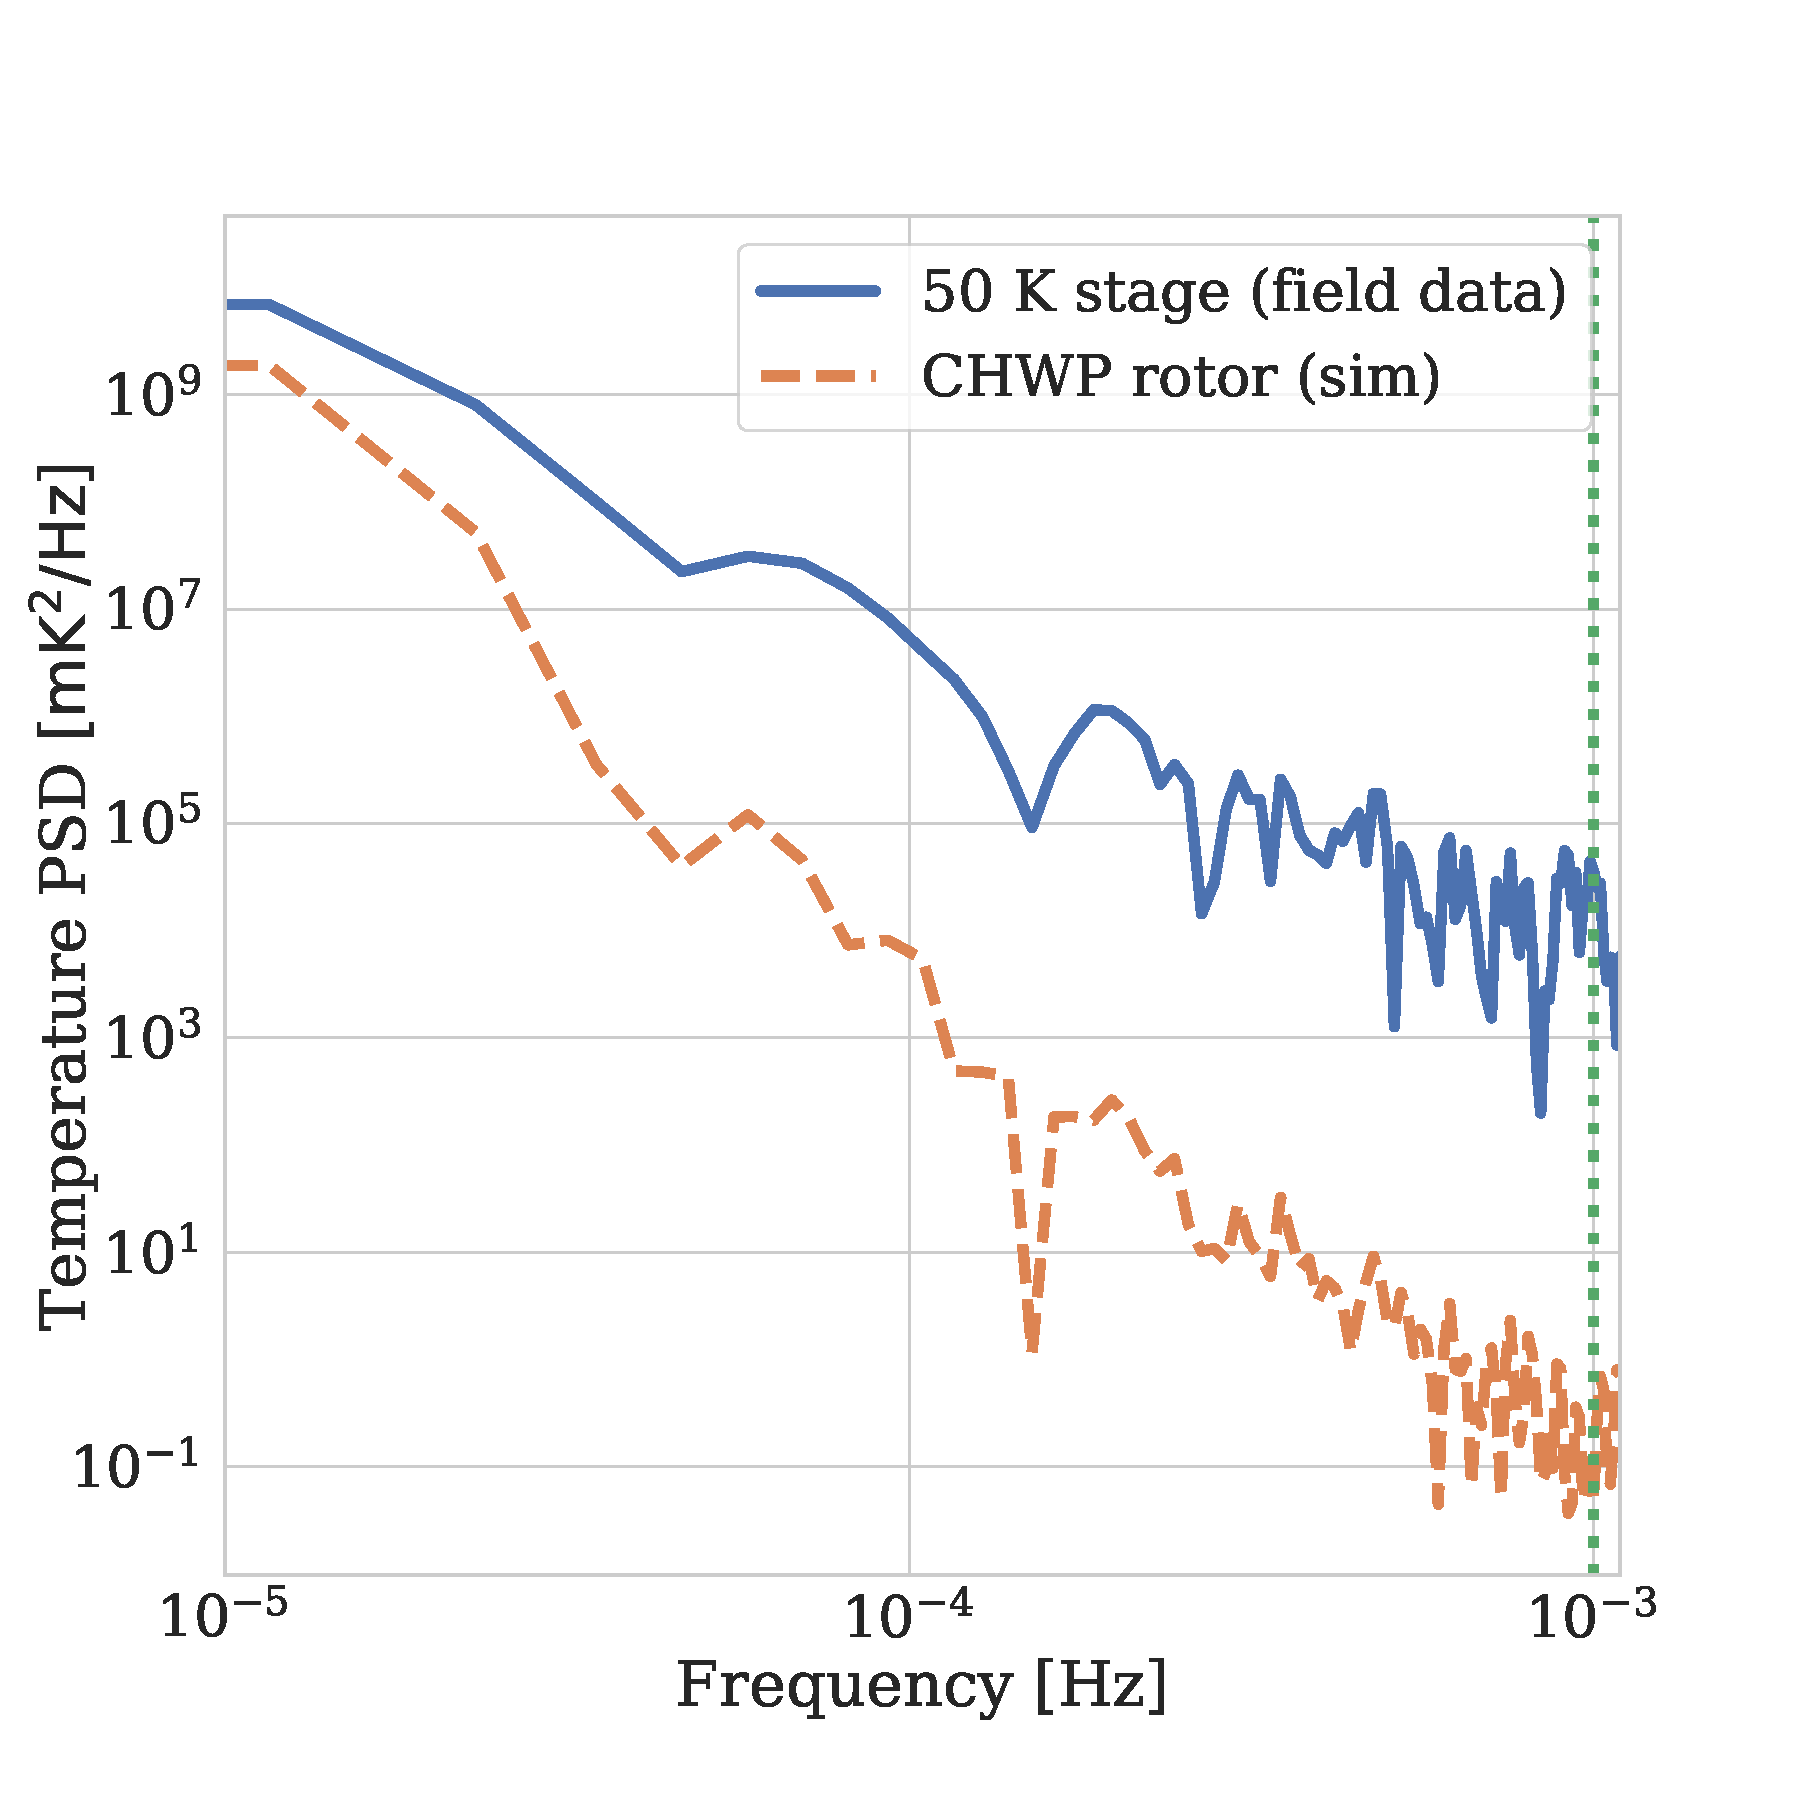
\includegraphics[width=0.48\linewidth, trim=0.3cm 1cm 2.4cm 3cm, clip]{CHWPEvaluation/Figures/rotor_tempVariation_pb2a_psd.pdf}
    \caption{Power spectra of measured 50~K temperature variations from PB-2a in Chile and of the resulting simulated rotor temperature variations. The rotor's large thermal mass and small radiative coupling make it an effective low-pass filter, suppressing IRF fluctuations by >~100$\times$ at 1~mHz.}
    \label{fig:hwp_stability}
\end{figure}
